\documentclass[11pt,reqno,a4letter]{article} 

\usepackage{amsmath,amssymb,amsfonts,amscd}

\usepackage{url}
\usepackage{hyperref}
\usepackage[usenames,dvipsnames]{xcolor}
\hypersetup{
    colorlinks,
    linkcolor={black!63!darkgray},
    citecolor={blue!70!white},
    urlcolor={blue!80!white}
}
\usepackage{graphicx} 

\usepackage{ocr}
\usepackage[T1]{fontenc}

\newcommand{\hlocalref}[1]{\hyperref[#1]{\ref{#1}}}

\usepackage{datetime} 
\usepackage{cancel}
\usepackage{soul} 
\usepackage{subcaption}
\captionsetup{format=hang,labelfont={bf},textfont={small,it}} 
\numberwithin{equation}{section} 
\numberwithin{figure}{section}
\numberwithin{table}{section}

\usepackage{tocloft}
\usepackage{framed} 

\usepackage{enumitem}
\setlist[itemize]{leftmargin=0.65in}

\usepackage{changepage}
\usepackage{rotating,adjustbox}

\usepackage{diagbox}
\newcommand{\trianglenk}[2]{$\diagbox{#1}{#2}$}
\newcommand{\trianglenkII}[2]{\diagbox{#1}{#2}}

\let\citep\cite

\newcommand{\undersetbrace}[2]{\underset{\displaystyle{#1}}{\underbrace{#2}}}

\newcommand{\gkpSI}[2]{\ensuremath{\genfrac{\lbrack}{\rbrack}{0pt}{}{#1}{#2}}} 
\newcommand{\gkpSII}[2]{\ensuremath{\genfrac{\lbrace}{\rbrace}{0pt}{}{#1}{#2}}}
\newcommand{\cf}{\textit{cf.\ }} 
\newcommand{\Iverson}[1]{\ensuremath{\left[#1\right]_{\delta}}} 
\newcommand{\floor}[1]{\left\lfloor #1 \right\rfloor} 
\newcommand{\ceiling}[1]{\left\lceil #1 \right\rceil} 
\newcommand{\e}[1]{e\left(#1\right)} 
\newcommand{\seqnum}[1]{\href{http://oeis.org/#1}{\color{ProcessBlue}{\underline{#1}}}}

\usepackage{upgreek,dsfont,amssymb}
\renewcommand{\chi}{\upchi}
\newcommand{\ChiFunc}[1]{\ensuremath{\chi_{\{#1\}}}}
\newcommand{\OneFunc}[1]{\ensuremath{\mathds{1}_{#1}}}

%\usepackage{mathabx}
\makeatletter
\newcommand*\rel@kern[1]{\kern#1\dimexpr\macc@kerna}
\newcommand*\widebar[1]{%
  \begingroup
  \def\mathaccent##1##2{%
    \rel@kern{0.8}%
    \overline{\rel@kern{-0.8}\macc@nucleus\rel@kern{0.2}}%
    \rel@kern{-0.2}%
  }%
  \macc@depth\@ne
  \let\math@bgroup\@empty \let\math@egroup\macc@set@skewchar
  \mathsurround\z@ \frozen@everymath{\mathgroup\macc@group\relax}%
  \macc@set@skewchar\relax
  \let\mathaccentV\macc@nested@a
  \macc@nested@a\relax111{#1}%
  \endgroup
}

\usepackage{MnSymbol}
\newcommand{\gkpEII}[2]{\ensuremath{\genfrac{\llangle}{\rrangle}{0pt}{}{#1}{#2}}}

\usepackage{ifthen}
\newcommand{\Hn}[2]{
     \ifthenelse{\equal{#2}{1}}{H_{#1}}{H_{#1}^{\left(#2\right)}}
}

\newcommand{\Floor}[2]{\ensuremath{\left\lfloor \frac{#1}{#2} \right\rfloor}}
\newcommand{\Ceiling}[2]{\ensuremath{\left\lceil \frac{#1}{#2} \right\rceil}}

\DeclareMathOperator{\DGF}{DGF} 
\DeclareMathOperator{\ds}{ds} 
\DeclareMathOperator{\Id}{Id}
\DeclareMathOperator{\fg}{fg}
\DeclareMathOperator{\Div}{div}
\DeclareMathOperator{\rpp}{rpp}
\DeclareMathOperator{\logll}{\ell\ell}

\title{
       \LARGE{
       Exact formulas for partial sums of the M\"obius function expressed by 
       partial sums weighted by the Liouville lambda function
       } 
}
\author{{\Large Maxie Dion Schmidt} \\[0.1cm]  
        {\normalsize \href{mailto:maxieds@gmail.com}{maxieds@gmail.com}} \\[0.025cm] 
        {\normalsize \href{mailto:mschmidt34@gatech.edu}{mschmidt34@gatech.edu}} \\[0.025cm] 
        {\normalsize Georgia Institute of Technology} \\[0.025cm] 
        {\normalsize School of Mathematics} 
} 

%\date{\small\underline{Last Revised:} \today \ @\ \hhmmsstime{} \ -- \ Compiled with \LaTeX2e} 

\usepackage{amsthm} 

\theoremstyle{plain} 
\newtheorem{theorem}{Theorem}
\newtheorem{conjecture}[theorem]{Conjecture}
\newtheorem{claim}[theorem]{Claim}
\newtheorem{prop}[theorem]{Proposition}
\newtheorem{lemma}[theorem]{Lemma}
\newtheorem{cor}[theorem]{Corollary}
\numberwithin{theorem}{section}
\newtheorem*{conjecture*}{Conjecture}

\theoremstyle{definition} 
\newtheorem{example}[theorem]{Example}
\newtheorem{remark}[theorem]{Remark}
\newtheorem{definition}[theorem]{Definition}
\newtheorem{notation}[theorem]{Notation}
\newtheorem{question}[theorem]{Question}
\newtheorem{discussion}[theorem]{Discussion}
\newtheorem{facts}[theorem]{Facts}
\newtheorem{summary}[theorem]{Summary}
\newtheorem{heuristic}[theorem]{Heuristic}
\newtheorem{observation}[theorem]{Observation}
\newtheorem{ansatz}[theorem]{Ansatz}

\renewcommand{\arraystretch}{1.25} 
\usepackage[total={7in, 9.5in},tmargin=0.75in,headsep=8pt,footskip=30pt,footnotesep=0.5in]{geometry}

\usepackage{fancyhdr}
\pagestyle{empty}
\pagestyle{fancy}
\fancyhead[RO,RE]{Maxie Dion Schmidt -- \today} 
\fancyhead[LO,LE]{}
\fancyheadoffset{0.005\textwidth} 

\setlength{\parindent}{0em}
\setlength{\parskip}{2.5em} 

\renewcommand{\thefootnote}{\textbf{\arabic{footnote}}}

\renewcommand{\Re}{\operatorname{Re}}
\renewcommand{\Im}{\operatorname{Im}}

\usepackage{tikz}
\usetikzlibrary{shapes,arrows}

\usepackage{longtable}
\usepackage{arydshln} 
\usepackage[symbols,nogroupskip,nomain,automake=true,nonumberlist,section=section]{glossaries-extra}
\usepackage{glossary-mcols} 

\defglsdisplayfirst[main]{#1#4\protect\footnote{#2}}

%%%%%%%%%%%%

\providecommand{\glossarytoctitle}{\glossaryname}
\setlength{\glsdescwidth}{0.7\textwidth}

\newglossarystyle{glossstyleSymbol}{%
\renewenvironment{theglossary}%
 {\begin{longtable}{lp{\glsdescwidth}}}%
 {\end{longtable}}%
 \setlength{\parskip}{3.5pt}
 \renewcommand{\glsgroupskip}{}
\renewcommand*\glspostdescription{\dotfill}
\renewcommand*{\glossaryheader}{%
 \bfseries Symbols & \bfseries Definition
 \\\endhead}%
 \renewcommand*{\glsgroupheading}[1]{}%
  \renewcommand{\glossentry}[2]{%
    \glstarget{##1}{\glossentrysymbol{##1}} &
    \glossentrydesc{##1} \tabularnewline
  }%
  \renewcommand*{\glspostdescription}{}
  \renewcommand{\glossarymark}[1]{}
}

\setglossarystyle{glossstyleSymbol}
\makeglossaries

%%%%%%%%%%%%

\newglossaryentry{fCvlg}{
    symbol={\ensuremath{f \ast g}},
    sort={fg},
    description={The Dirichlet convolution of any two arithmetic functions 
    $f$ and $g$ at $n$ is defined to be 
    the divisor sum $(f \ast g)(n) := \sum\limits_{d|n} f(d) g\left(\frac{n}{d}\right)$ 
    for $n \geq 1$. 
    },
    type={symbols},
    name={Dirichlet convolution}
    }
%\newglossaryentry{coeffExtraction}{
%    symbol={\ensuremath{[q^n] F(q)}},
%    sort={coeffExtraction},
%    description={The coefficient of $q^n$ in the power series expansion of $F(q)$ about zero when 
%    $F(q)$ is treated as the ordinary generating function (OGF) of a sequence, $\{f_n\}_{n \geq 0}$. 
%    Namely, for integers $n \geq 0$ we define $[q^n] F(q) = f_n$ whenever 
%    $F(q) := \sum\limits_{n \geq 0} f_n q^n$. },
%    type={symbols},
%    name={Series coefficient extraction}
%    }
\newglossaryentry{MoebiusMuFunc}{
    symbol={\ensuremath{\mu(n),M(x)}},
    sort={MoebiusMuFunc},
    description={The M\"obius function defined such that $\mu^2(n)$ is the indicator function of the 
                 squarefree integers $n \geq 1$ where 
                 $\mu(n) = (-1)^{\omega(n)}$ whenever $n$ is squarefree. 
                 The Mertens function is the summatory function defined for all integers 
                 $x \geq 1$ by the partial sums $M(x) := \sum\limits_{n \leq x} \mu(n)$.
                 },
    type={symbols},
    name={M\"obius function}
    }
\newglossaryentry{Iverson}{
    symbol={\ensuremath{\Iverson{n=k}},\ensuremath{\Iverson{\mathtt{cond}}}},
    sort={Iverson},
    description={The symbol $\Iverson{n=k}$ is a synonym for $\delta_{n,k}$ 
                 which is one if and only if $n = k$, and is zero otherwise. 
                 For Boolean-valued conditions, \texttt{cond}, the symbol $\Iverson{\mathtt{cond}}$ 
                 evaluates to one precisely when \texttt{cond} is true or to zero otherwise.},
    type={symbols},
    name={Iverson's convention}
    }
\newglossaryentry{epsilonN}{
    symbol={\ensuremath{\varepsilon(n)}},
    sort={epsilonN},
    description={The multiplicative identity with respect to Dirichlet convolution, $\varepsilon(n) := \delta_{n,1}$, 
                 defined such that for any arithmetic function $f$ we have that 
                 $f \ast \varepsilon = \varepsilon \ast f = f$ where the operation 
                 $\ast$ denotes Dirichlet convolution. },
    type={symbols},
    name={Dirichlet multiplicative identity}
    }
\newglossaryentry{Zetas}{
    symbol={\ensuremath{\zeta(s)}},
    sort={Zetas},
    description={The Riemann zeta function is defined by 
                 $\zeta(s) := \sum\limits_{n \geq 1} n^{-s}$ when $\Re(s) > 1$, 
                 and by analytic continuation to any $s \in \mathbb{C}$ with the exception of a 
                 simple pole at $s = 1$ of residue one.},
    type={symbols},
    name={Riemann zeta function}
    }
\newglossaryentry{fInvn}{
     symbol={\ensuremath{f^{-1}(n)}},
    sort={fInvn},
    description={
     The Dirichlet inverse $f^{-1}$ of an arithmetic function $f$ exists 
     if and only if $f(1) \neq 0$. 
     The Dirichlet inverse of any $f$ such that $f(1) \neq 0$ 
     is defined recursively by 
     $f^{-1}(n) = -\frac{1}{f(1)} \times \sum\limits_{\substack{d|n \\ d>1}} f(d) f^{-1}\left(\frac{n}{d}\right)$ 
     for $n \geq 2$ with $f^{-1}(1) = f(1)^{-1}$. 
     When it exists, this inverse function 
     is unique and satisfies  $f^{-1} \ast f = f \ast f^{-1} = \varepsilon$.},
    type={symbols},
    name={Dirichlet inverse of $f$}
    }
\newglossaryentry{CkngInvAuxFunc}{
    symbol={$C_k(n),C_{\Omega}(n)$},
    sort={CkngInvAuxFunc},
    description={The first sequence is defined recursively for integers $n \geq 1$ and $k \geq 0$ as follows: 
                 \[
                 C_k(n) := \begin{cases} 
                      \delta_{n,1}, & \text{ if $k = 0$; } \\ 
                      \sum\limits_{d|n} \omega(d) C_{k-1}\left(\frac{n}{d}\right), & \text{ if $k \geq 1$. } 
                      \end{cases} 
                 \]
                 It represents the multiple ($k$-fold) convolution of the function $\omega(n)$ 
                 with itself. 
                 The function $C_{\Omega}(n) := C_{\Omega(n)}(n)$ has the DGF 
                 $(1-P(s))^{-1}$ for $\Re(s) > 1$. 
                 },
    type={symbols},
    name={Dirichlet inverse component functions}
    }
\newglossaryentry{gInvn}{
    symbol={$g(n),G(x),|G|(x)$},
    sort={gInvn},
    description={The Dirichlet inverse function, $g(n) = (\omega+1)^{-1}(n)$, has the 
                 summatory function $G(x) := \sum\limits_{n \leq x} g(n)$ for $x \geq 1$. 
                 We define the partial sums of the unsigned inverse function to be 
                 $|G|(x) := \sum_{n \leq x} |g(n)|$ for $x \geq 1$. },
    type={symbols},
    name={Key Dirichlet inverse functions}
    }
\newglossaryentry{PikPiHatkx}{
    symbol={$\pi_k(x),\widehat{\pi}_k(x)$},
    sort={PikPiHatkx},
    description={For integers $k \geq 1$, the 
                 function $\pi_k(x)$ denotes the number of 
                 $2 \leq n \leq x$ with 
                 exactly $k$ distinct prime factors: $\pi_k(x) := \#\{2 \leq n \leq x: \omega(n) = k\}$. 
                 Similarly, the function 
                 $\widehat{\pi}_k(x) := \#\{2 \leq n \leq x: \Omega(n) = k\}$ for $x \geq 2$ and fixed $k \geq 1$. },
    type={symbols},
    name={Distinct prime counting functions}
    }   
\newglossaryentry{primeOmegaFunctions}{
    symbol={$\omega(n)$,$\Omega(n)$}, 
    sort={OmegaPrimeOmegaFunctions},
    description={We define the strongly additive function 
                 $\omega(n) := \sum\limits_{p|n} 1$ and the completely additive function 
                 $\Omega(n) := \sum\limits_{p^{\alpha} || n} \alpha$. This means that if the prime 
                 factorization of any $n \geq 2$ is 
                 given by $n := p_1^{\alpha_1} \times \cdots \times p_r^{\alpha_r}$ 
                 with $p_i \neq p_j$ for all $i \neq j$, 
                 then $\omega(n) = r$ and $\Omega(n) = \alpha_1 + \cdots + \alpha_r$. 
                 We set $\omega(1) = \Omega(1) = 0$ by convention.},
    type={symbols},
    name={Prime omega functions}
    }
\newglossaryentry{LiouvilleLambdaFunc}{
     symbol={$\lambda(n), L(x)$}, 
    sort={LiouvilleLambdaFunc},
    description={The Liouville lambda function is the completely multiplicative function defined by 
                 $\lambda(n) := (-1)^{\Omega(n)}$. 
                 Its summatory function is defined by the partial sums 
                 $L(x) := \sum\limits_{n \leq x} \lambda(n)$ for $x \geq 1$. 
                 },
    type={symbols},
    name={Liouville lambda function}
    }
\newglossaryentry{QxSummatoryFunc}{
    symbol={$Q(x)$},
    sort={QxSummatoryFunc},
    description={For $x \geq 1$, we define $Q(x)$ to be the summatory function indicating the number of 
		 squarefree integers $n \leq x$. That is, $Q(x) = \sum_{n \leq x} \mu^2(n)$ for $x \geq 1$. }, 
    type={symbols},
    name={Summatory function of the squarefree integers}
    }
\newglossaryentry{AApproxSimGGLLRelations}{
    symbol={$\gg,\ll,\asymp,\sim$},
    sort={AApproxSimGGLLRelations},
    description={
                 For functions $A,B$, the notation $A \ll B$ implies that $A = O(B)$. 
                 Similarly, for $B \geq 0$ the notation $A \gg B$ implies that $B = O(A)$. 
                 When we have that $A, B \geq 0$, $A \ll B$ and $B \ll A$, we write $A \asymp B$. 
                 Two arithmetic functions $A(x), B(x)$ satisfy the relation $A \sim B$ if 
                 $\lim_{x \rightarrow \infty} \frac{A(x)}{B(x)} = 1$. },
    type={symbols},
    name={Asymptotic relation symbols}
    }
\newglossaryentry{chiPrimeP}{
    symbol={$\chi_{\mathbb{P}}(n), P(s)$},
    sort={chiPrimeP},
    description={The indicator function of the primes equals one if and only if 
                 $n \in \mathbb{Z}^{+}$ is prime and is defined to be 
                 zero-valued otherwise. 
                 For any $s \in \mathbb{C}$ such that $\Re(s) > 1$, 
                 we define the prime zeta function to be the 
                 Dirichlet generating function (DGF) defined by 
		 $P(s) = \sum\limits_{n \geq 1} \chi_{\mathbb{P}}(n) n^{-s}$. 
                 The function $P(s)$ has an analytic continuation to the half-plane 
                 $\Re(s) > 0$ with the exception of $s = 1$ through the formula 
                 $P(s) = \sum\limits_{k \geq 1} \frac{\mu(k)}{k} \log\zeta(ks)$. The DGF $P(s)$ 
                 poles at the reciprocal of each positive integer and a natural boundary 
                 at the line $\Re(s) = 0$. },
    type={symbols},
    name={Prime set indicator function}
    }
\newglossaryentry{WLambertWFunction}{
    symbol={$W(x)$},
    sort={WLambertWFunction},
    description={For $x,y \in [0, \infty)$, we write that $x = W(y)$ if and only if $xe^{x} = y$. 
                 This function denotes the principal branch of the multi-valued Lambert $W$ function 
                 taken over the non-negative reals. },
    type={symbols},
    name={Lambert $W$-Function}
    }
\newglossaryentry{GammaIncompleteGamma}{
    symbol={$\Gamma(a, z)$},
    sort={GammaIncompleteGamma},
    description={The incomplete gamma function is defined as $\Gamma(a, z) := \int_z^{\infty} t^{a-1} e^{-t} dt$ 
		 by continuation for $a \in \mathbb{R}$ and $|\operatorname{arg}(z)| < \pi$. }, 
    type={symbols},
    name={Incomplete gamma function}
    }
\newglossaryentry{NormalCDFFunc}{
    symbol={$\Phi(z)$},
    sort={NormalCDFFunc},
    description={For $z \in \mathbb{R}$, we take the cumulative density function 
                 of the standard normal distribution to be denoted by 
                 $\Phi(z) := \frac{1}{\sqrt{2\pi}} \times \int\limits_{-\infty}^{z} e^{-\frac{t^2}{2}} dt$. 
                },
    type={symbols},
    name={Asymptotic relation symbol}
    }

\glsaddall[types={symbols}]

\allowdisplaybreaks 

\begin{document} 

\maketitle
\newcommand{\runtitle}{New formulas for partial sums of the M\"obius function}
\lhead{Maxie Dion Schmidt \hspace{0.65cm} -- \small{\today} --}
\rhead{\runtitle}

\begin{abstract} 
\noindent  
The Mertens function, $M(x) := \sum_{n \leq x} \mu(n)$, is 
defined as the summatory function of the classical M\"obius function for $x \geq 1$.
The Dirichlet inverse function $g(n) := (\omega+\mathds{1})^{-1}(n)$
is defined in terms of the shifted strongly additive function $\omega(n)$ that counts the 
number of distinct prime factors of $n$ without multiplicity. 
Discrete convolutions of the partial sums of $g(n)$ with the prime counting function 
provide new exact formulas for $M(x)$ that are weighted sums of the Liouville function 
multiplied by the unsigned summands $|g(n)|$ for $n \leq x$. 
We study the distribution of the unsigned function $|g(n)|$ whose 
Dirichlet generating function (DGF) is $\zeta(2s)^{-1}(1-P(s))^{-1}$ 
through the auxiliary unsigned sequence $C_{\Omega}(n)$ whose DGF is given by 
$(1-P(s))^{-1}$ for $\Re(s) > 1$ where $P(s) = \sum_p p^{-s}$ is the 
prime zeta function. 
We prove formulas for the average order and variance of both 
$\log C_{\Omega}(n)$ and $\log |g(n)|$ and conjecture a central limit theorem 
for the distribution of their values over $n \leq x$ as $x \rightarrow \infty$. 

\bigskip 
\noindent
\textbf{Keywords and Phrases:} {\it M\"obius function; Mertens function; 
                                    Dirichlet inverse; Liouville lambda function; prime omega function; 
                                    prime counting function; Dirichlet generating function; 
                                    prime zeta function. } \\ 
% 11-XX			Number theory
%    11A25  	Arithmetic functions; related numbers; inversion formulas
%    11Y70  	Values of arithmetic functions; tables
%    11-04  	Software, source code, etc. for problems pertaining to number theory
% 11Nxx		Multiplicative number theory
%    11N05  	Distribution of primes
%    11N37  	Asymptotic results on arithmetic functions
%    11N56  	Rate of growth of arithmetic functions
%    11N60  	Distribution functions associated with additive and positive multiplicative functions
%    11N64  	Other results on the distribution of values or the characterization of arithmetic functions
\textbf{Math Subject Classifications (2010):} {\it 11N37; 11A25; 11N60; 11N64; and 11-04. } 
\end{abstract} 

\newpage
\renewcommand{\contentsname}{Table of Contents}
\setcounter{tocdepth}{2}
\tableofcontents

\newpage
\section{Introduction} 
\label{subSection_MertensMxClassical_Intro} 
\label{example_InvertingARecRelForMx_Intro}

\subsection{Definitions}

For integers $n \geq 2$, we define the strongly and 
completely additive functions, respectively, 
that count the number of prime divisors of $n$ by 
\begin{align*}
\omega(n) & = \sum_{p|n} 1, \text{ and } 
     \Omega(n) = \sum_{p^{\alpha} \mid\mid n} \alpha. 
\end{align*}
We use the convention that when $n = 1$, the functions $\omega(1) = \Omega(1) = 0$. 
The M\"obius function is defined as the signed indicator function of the squarefree integers by 
\[
\mu(n) = \begin{cases} 
	1, & \text{ if $n = 1$}; \\ 
	(-1)^{\omega(n)}, & \text{ if $n \geq 2$ and $\omega(n) = \Omega(n)$;} \\ 
	0, & \text{ otherwise.}
        \end{cases}
\]
The Mertens function is the summatory function defined by the partial sums 
\cite[\seqnum{A008683}; \seqnum{A002321}]{OEIS} 
\begin{align} 
M(x) & = \sum_{n \leq x} \mu(n), \text{ for } x \geq 1. 
\end{align} 
The Liouville lamda function is defined for all $n \geq 1$ by $\lambda(n) := (-1)^{\Omega(n)}$. 
The partial sums of this function are defined by 
\cite[\seqnum{A008836}; \seqnum{A002819}]{OEIS}
\begin{equation}
\label{eqn_LxSummatoryFuncDef_v1}
L(x) := \sum\limits_{n \leq x} \lambda(n), \text{ for } x \geq 1. 
\end{equation}
For any arithmetic functions $f$ and $h$, we define their Dirichlet convolution at $n \geq 1$ by 
\[
(f \ast h)(n) := \sum_{d|n} f(d) h\left(\frac{n}{d}\right).
\]
The arithmetic function $f$ has a unique inverse with respect to Dirichlet convolution, 
denoted by $f^{-1}$, that satisfies $(f \ast f^{-1})(n) = (f^{-1} \ast f)(n) = \delta_{n,1}$ 
if and only if $f(1) \neq 0$. 
We define the Dirichlet inverse \cite[\seqnum{A341444}]{OEIS} 
\begin{equation}
\label{eqn_gInvn_def_v1}
g(n) := (\omega + \mathds{1})^{-1}(n), \text{ for } n \geq 1. 
\end{equation}
This Dirichlet inverse function is computed recursively for any $n \geq 1$ 
by the formula \cite[\S 2.7]{APOSTOLANUMT}
\[
g(n) = \begin{cases}
	1, & \text{ if $n = 1$; } \\ 
	-\sum\limits_{\substack{d|n \\ d> 1}} \left(\omega(d) + 1\right) g\left(\frac{n}{d}\right), & 
	\text{ if $n \geq 2$. }
        \end{cases}
\]
We let $|g(n)| = \lambda(n) g(n)$ denote the absolute value of $g(n)$ 
(see Proposition \hlocalref{prop_SignageDirInvsOfPosBddArithmeticFuncs_v1}). 
The partial sums of $g(n)$ are defined for integers $x \geq 1$ as follows 
\cite[\seqnum{A341472}]{OEIS}: 
\begin{equation}
\label{eqn_GInvx_PartialSumForms_v1} 
G(x) := \sum_{n \leq x} g(n) = \sum_{n \leq x} \lambda(n) |g(n)|. 
\end{equation} 

\subsection{Statements of the main results}

For any $x \geq 1$, the function $\pi(x) := \sum_{p \leq x} 1$ 
in the next theorem denotes the classical prime counting function.

\begin{theorem} 
\label{prop_Mx_SBP_IntegralFormula} 
\begin{subequations}
For all $x \geq 1$ 
\begin{align} 
\label{prop_Mx_SBP_IntegralFormula_PartA} 
M(x) & = G(x) + \sum_{1 \leq k \leq x} |g(k)| \pi\left(\Floor{x}{k}\right) \lambda(k), \\ 
\label{prop_Mx_SBP_IntegralFormula_PartB} 
M(x) & = G(x) + 
     \sum_{1 \leq k \leq \frac{x}{2}} \left(
     \pi\left(\Floor{x}{k}\right) - \pi\left(\Floor{x}{k+1}\right) 
	\right) G(k), \\ 
\label{eqn_RmkInitialConnectionOfMxToGInvx_ProvedByInversion_v1} 
M(x) & = G(x) + \sum_{p \leq x} G\left(\Floor{x}{p}\right). 
\end{align} 
\end{subequations}
\end{theorem}

An exact expression for $g(n)$ involving the auxiliary function 
$C_{\Omega}(n)$ is given by 
(see Lemma \hlocalref{lemma_AnExactFormulaFor_gInvByMobiusInv_v1} and 
Corollary \hlocalref{lemma_AbsValueOf_gInvn_FornSquareFree_v1}) 
\begin{equation}
\label{eqn_gInvn_ExactDivisorSumFormula_WithSgnWeight_v1} 
\lambda(n) g(n) = \sum_{d|n} \mu^2\left(\frac{n}{d}\right) C_{\Omega}(d), n \geq 1. 
\end{equation}
The sequence $\lambda(n) C_{\Omega}(n)$ has the 
Dirichlet generating function (DGF) of $(1 + P(s))^{-1}$ and 
$C_{\Omega}(n)$ has the DGF $(1-P(s))^{-1}$ for $\Re(s) > 1$ 
where $P(s) := \sum_p p^{-s}$ is the prime zeta function. 
The function $C_{\Omega}(n)$ was considered in 
\cite{FROBERG-1968} with an exact formula given by 
(\cf equation \eqref{eqn_COmeganMultinomExp_as_DGFSeries_v2} in the 
proof of Proposition \hlocalref{prop_SignageDirInvsOfPosBddArithmeticFuncs_v1}) 
\begin{equation}
\label{eqn_proof_tag_hInvn_ExactNestedSumFormula_CombInterpetIdent_v3}
C_{\Omega}(n) = \begin{cases}
     1, & \text{if $n = 1$; } \\ 
     (\Omega(n))! \times \prod\limits_{p^{\alpha}||n} \frac{1}{\alpha!}, & \text{if $n \geq 2$. }
     \end{cases}
\end{equation} 
The DGF of $g(n)$ is given by $\zeta(s)^{-1} (1 + P(s))^{-1}$ for $\Re(s) > 1$ 
(see Proposition \hlocalref{prop_SignageDirInvsOfPosBddArithmeticFuncs_v1}). 
The DGF of $|g(n)|$ is given by $\zeta(2s)^{-1} (1 - P(s))^{-1}$ for $\Re(s) > 1$ 
(see Remark \hlocalref{remark_MiscConsequencesOfCorForFormulaOfUnsgInvnFunc_v2}). 

\begin{theorem} 
\label{lemma_HatCAstxSum_ExactFormulaWithError_v1} 
As $n \rightarrow \infty$, there is an absolute constant $B_0 > 0$ such that
\[
\frac{1}{n} \times \sum_{k \leq n} \log C_{\Omega}(k) = 
     B_0 (\log\log n)(\log\log\log n) \left(1 + o(1)\right). 
\] 
\end{theorem} 

\begin{conjecture*}
For any fixed $z > 0$, as $x \rightarrow \infty$ 
\begin{align*} 
\frac{1}{x} \times \#\left\{2 \leq n \leq x: -z \leq |g(n)| - 
     \frac{1}{n} \times \sum_{k \leq n} |g(k)| \leq z\right\} & = 
	\Phi\left(\frac{\log\left(\frac{\pi^2 z}{6}\right) - B_0 \cdot (\log\log x) (\log\log\log x)}{ 
	B_0 \cdot (\log\log x)(\log\log\log x)}\right) + o(1).
\end{align*} 
\end{conjecture*}

We can show that the constant $B_0$ in the conjecture is 
identically one assuming that for any fixed, finite $y > 0$ 
\begin{align*} 
	\frac{1}{x} \times \#\left\{2 \leq n \leq x: 
	\frac{C_{\Omega}(n)}{ (\log\log x)(\log\log\log x)} \leq y\right\} & = 
	\Phi\left(y - 1\right) + o(1), \text{ as } x \rightarrow \infty.
\end{align*} 

\subsection{Discussion of the new results}

For $n \geq 2$, let the function 
$\mathcal{E}[n] := (\alpha_1, \alpha_2, \ldots, \alpha_r)$ denote the unordered 
partition of exponents for which 
$n = p_1^{\alpha_1} \times \cdots \times p_r^{\alpha_r}$ is the factorization of 
$n$ into powers of distinct primes. 
For any $n_1,n_2 \geq 2$ 
\begin{equation}
\label{eqn_FactSymmPropertyOfgn_v1} 
\mathcal{E}[n_1] = \mathcal{E}[n_2] \implies C_{\Omega}(n_1) = C_{\Omega}(n_2) \text{ and } 
	g(n_1) = g(n_2). 
\end{equation}
The Mertens function is related to the partial sums in 
\eqref{eqn_LxSummatoryFuncDef_v1} 
via the relation \cite{HUMPHRIES-JNT-2013,LEHMAN-1960} 
\begin{equation}
\label{eqn_MxInTermsOfLx_v1} 
M(x) = \sum_{d \leq \sqrt{x}} \mu(d) L\left(\Floor{x}{d^2}\right), \text{ for } x \geq 1.
\end{equation}
The relation in \eqref{eqn_MxInTermsOfLx_v1} 
gives an exact expression for $M(x)$ with summands involving $L(x)$ that are oscillatory. 
In contrast, the exact expansions for the Mertens function given in 
Theorem \hlocalref{prop_Mx_SBP_IntegralFormula} 
express $M(x)$ as finite sums over $\lambda(n)$ with weighted coefficients that are unsigned. 
The property of the symmetry of the distinct values of $|g(n)|$ with respect to the 
prime factorizations of $n \geq 2$ in \eqref{eqn_FactSymmPropertyOfgn_v1} 
suggests that the unsigned weights on $\lambda(n)$ in 
the new formulas from the theorem yield new insights compared to the 
formula for $M(x)$ in terms of $L(x)$ from equation \eqref{eqn_MxInTermsOfLx_v1}.

\subsection{Organization of the manuscript}

The focus of the article is on the unsigned functions 
$C_{\Omega}(n)$ and $|g(n)|$. 
The new formulas for $M(x)$ given in 
Theorem \hlocalref{prop_Mx_SBP_IntegralFormula} 
provide a window from which we can view classically  
difficult problems about asymptotics for this function in terms of the 
auxiliary unsigned functions. 
We first prove formulas for the first and second moments of the functions 
$C_{\Omega}(n)$ and $g(n)$. We then establish the proof of 
Theorem \hlocalref{prop_Mx_SBP_IntegralFormula} in 
Section \hlocalref{Section_KeyApplications}. 
The appendix sections provide 
supplementary material on topics that can be separated from the 
main sections of the article. 

\section{Properties of the function $C_{\Omega}(n)$} 
\label{Section_NewFormulasForgInvn_v1} 

The function $C_{\Omega}(n)$ is key to understanding the 
unsigned inverse sequence $|g(n)|$ through equation 
\eqref{eqn_gInvn_ExactDivisorSumFormula_WithSgnWeight_v1}. 
In this section, we define the function 
$C_{\Omega}(n)$ and explore its properties. 

\subsection{Definitions}

\begin{definition}
We define the following bivariate sequence for integers $n \geq 1$ and $k \geq 0$: 
\begin{align} 
\label{eqn_CknFuncDef_v2} 
C_k(n) := \begin{cases} 
     \varepsilon(n), & \text{ if $k = 0$; } \\ 
     \sum\limits_{d|n} \omega(d) C_{k-1}\left(\frac{n}{d}\right), & \text{ if $k \geq 1$. } 
     \end{cases} 
\end{align} 
Using the notation for iterated convolution in 
Bateman and Diamond \cite[Def.~ 2.3; \S 2]{ANT-BATEMAN-DIAMOND}, we have 
$C_0(n) \equiv \omega^{\ast 0}(n)$ and $C_k(n) \equiv \omega^{\ast k}(n)$ for 
integers $k \geq 1$ and $n \geq 1$. 
The special case of \eqref{eqn_CknFuncDef_v2} where 
$k := \Omega(n)$ occurs frequently in the next sections of the 
article. To avoid cumbersome notation when referring to this common function variant, we suppress the 
duplicate index $n$ by writing $C_{\Omega}(n) := C_{\Omega(n)}(n)$ \cite[\seqnum{A008480}]{OEIS}. 
\end{definition}

\begin{remark}
By recursively expanding the definition of $C_k(n)$ 
at any fixed $n \geq 2$, we see that 
we can form a chain of at most $\Omega(n)$ iterated (or nested) divisor sums by 
unfolding the definition of \eqref{eqn_CknFuncDef_v2} inductively. 
We also see that at fixed $n$, the function 
$C_k(n)$ is non-zero only possibly for 
$1 \leq k \leq \Omega(n)$ when $n \geq 2$. 
By \eqref{eqn_proof_tag_hInvn_ExactNestedSumFormula_CombInterpetIdent_v3} we have 
that $C_{\Omega}(n) \leq (\Omega(n))!$ for all $n \geq 1$ with 
equality precisely at the squarefree integers so that 
$(\Omega(n))! = (\omega(n))!$ if and only if $\mu^2(n) = 1$. 
\end{remark}

\subsection{Average order and variance}
\label{subSection_AvgOrdersOfTheUnsignedSequences} 

\begin{proof}[Proof of Theorem \hlocalref{lemma_HatCAstxSum_ExactFormulaWithError_v1}]  
We first use \eqref{eqn_proof_tag_hInvn_ExactNestedSumFormula_CombInterpetIdent_v3} to 
see that there is an absolute constant $P_0 \geq \frac{6}{\pi^2}$ such that 
\begin{align}
\label{eqn_proof_tag_SumLogCOmegan_P0_exp_v1}
\sum_{k \geq 1} \sum_{\substack{n \leq x \\ \Omega(n)=k}} \log C_{\Omega}(n) & = 
	\sum_{k \geq 1} P_0 \times \#\{n \leq x: \Omega(n)=k\} \times \log(k!) (1 + o(1)). 
\end{align}
A complete proof that equation 
\eqref{eqn_proof_tag_SumLogCOmegan_P0_exp_v1} holds is given below.
We will split the full sum on the left-hand-side of 
\eqref{eqn_proof_tag_SumLogCOmegan_P0_exp_v1} into two sums over disjoint indices 
that form the main and error terms in the theorem.
For $x \geq 3$, consider the following partial sums:
\[
L_{\Omega}(x) := \sum_{1 \leq k \leq \frac{3}{2}\log\log x} 
	\sum_{\substack{n \leq x \\ \Omega(n)=k}} \log C_{\Omega}(n). 
\]
For any $z \geq 0$, we cite 
Binet's formula for the log-gamma function stated as follows 
\cite[\S 5.9(i)]{NISTHB}: 
\[
\log z! = \left(z+\frac{1}{2}\right)\log(1+z) - z + O(1). 
\]
If \eqref{eqn_proof_tag_SumLogCOmegan_P0_exp_v1} holds, 
Theorem \ref{theorem_HatPi_ExtInTermsOfGz} 
(see appendix) shows that there is an absolute constant $B_0 > 0$ such that 
\begin{align}
\label{eqn_proof_tag_SumLogCOmegan_P0_exp_v2}
L_{\Omega}(x) & = \sum_{1 \leq k \leq \frac{3}{2}\log\log x} 
	\frac{B_0 x (\log\log x)^{k-1}}{(\log x) (k-1)!} \times \left(
	\left(k+\frac{1}{2}\right) \log(1+k) - k\right)\left(1 + o(1)\right). 
\end{align}
The right-hand-side of \eqref{eqn_proof_tag_SumLogCOmegan_P0_exp_v2} can be 
approximated by Abel summation using the functions 
\[
A_x(u) := \frac{B_0 x \Gamma\left(u, \log\log x\right)}{\Gamma\left(u\right)}; 
     f(u) := \frac{(2u+1)}{2} \log\left(1 + u\right) - \frac{(2u+1)}{2}, 
     f^{\prime}(u) = \log\left(1 + u\right) - \frac{1}{2\left(1 + u\right)}. 
\]
We have by Proposition \hlocalref{prop_IncGammaLambdaTypeBounds_v1} that 
\begin{align*}
L_{\Omega}(x) & = A_x\left(\frac{3}{2}\log\log x\right) f\left(\frac{3}{2}\log\log x\right) - 
	\int_0^{\frac{3}{2}} A_x(\alpha \log\log x) f^{\prime}(\alpha \log\log x) d\alpha \\ 
	& = 
	B_0 x (\log\log x)(\log\log\log x) \left(1 + o(1)\right). 
\end{align*}
It suffices to show that 
\begin{equation}
\label{eqn_proof_tag_PartialSumsOver_HatCkx_EquivCond_v2}
\sum_{\substack{n \leq x \\ \Omega(n) \geq \frac{3}{2} \log\log x}} 
	\log C_{\Omega}(n)= o\left(x (\log\log x) (\log\log\log x)\right), 
	\text{ as } x \rightarrow \infty. 
\end{equation}
Because $r-1-r\log r \approx -0.108198$ when $r := \frac{3}{2}$ and 
\begin{equation}
\label{eqn_proof_tag_LogCOmegan_ll_FuncOfOmegan_v1}
\log C_{\Omega}(n) \ll \Omega(n) \log \Omega(n), \text{ for } n \leq x,
\end{equation}
we can argue using Rankin's method \cite[Thm.~7.20; \S 7.4]{MV} that 
\eqref{eqn_proof_tag_PartialSumsOver_HatCkx_EquivCond_v2} holds. 
In particular, the bounds provided in 
Theorem \hlocalref{theorem_MV_Thm7.20-init_stmt} 
together with applications of the Cauchy-Schwarz and 
the (logarithmic) AGM inequalities fill in the 
complete details to a proof verifying that the bound in 
\eqref{eqn_proof_tag_PartialSumsOver_HatCkx_EquivCond_v2} 
is attained at all sufficiently large $x$. 
The assertion on the upper bound for $\log C_{\Omega}(n)$ in 
\eqref{eqn_proof_tag_LogCOmegan_ll_FuncOfOmegan_v1} holds 
for all $n \geq 1$ even when the right-hand-side terms involving $\Omega(n)$ 
oscillate in magnitude over $1 \leq n \leq x$. This is justified by 
maximizing (minimizing) the ratio of the right-hand-side of 
\eqref{eqn_proof_tag_LogCOmegan_ll_FuncOfOmegan_v1} to 
Binet's log-gamma formula numerically to find explicit bounded real 
$z \equiv \Omega(n) \in [1, 11)$ 
that yield the extrema of the function.
\end{proof} 

\begin{proof}[Proof of equation \eqref{eqn_proof_tag_SumLogCOmegan_P0_exp_v1}]
The key to this argument is in understanding that the main term of the 
sum on the left-hand-side of the equation is obtained by summing over only 
the squarefree $n \leq x$. We claim that 
\[
\sum_{k \geq 1} \sum_{\substack{n \leq x \\ \Omega(n)=k}} \log C_{\Omega}(n) \sim 
	\sum_{k \geq 1} \sum_{\substack{n \leq x \\ \mu^2(n) = 1 \\ \Omega(n)=k}} \log C_{\Omega}(n). 
\]
For integers $x \geq 1$ and $1 \leq k \leq \log_2(x)$, let the sets 
\[
\mathcal{S}_k\left(\{\varpi_j\}_{j=1}^k; x\right) := \left\{2 \leq n \leq x: \mu(n) = 0, \omega(n) = k, 
	\frac{n}{\operatorname{rad}(n)} = p_1^{\varpi_1} \times \cdots \times p_k^{\varpi_k}, 
	\text{ $p_i \neq p_j$ prime if $1 \leq i < j \leq k$ }\right\}. 
\]
The function $\operatorname{rad}(n)$ is the radix of $n$ which evaluates 
to the largest squarefree factor of $n$, 
or equivalently the product of all primes $p | n$. 
Let $$\mathcal{N}_k(\varpi_1, \ldots, \varpi_k; x) := 
	\frac{\left\lvert \mathcal{S}_k\left(\{\varpi_j\}_{j=1}^k; x\right) \right\rvert}{x}.$$ 
Let the special case where $\{\varpi_j\}_{1 \leq j \leq k} \equiv \{1\}$ 
(with multiplicity of exactly one) be denoted by 
$$\widehat{T}_k(x) := \mathcal{N}_k(1, 0, \ldots, 0; x).$$ 
If $2 \leq n \leq x$ is not squarefree and $n \in \mathcal{S}_k\left(\{\varpi_j\}_{j=1}^k; x\right)$, then 
we must have that $\varpi_j \geq 1$ for at least one $1 \leq j \leq k$. 
We clearly have that for any $k \geq 1$ and non-trivial 
$\{\varpi_j\}_{1 \leq j \leq k} \neq \{0\}$ 
\[
\lim_{x \rightarrow \infty} \mathcal{N}_k(\varpi_1, \ldots, \varpi_k; x) \leq 
     \lim_{x \rightarrow \infty} \binom{k}{1} \times \widehat{T}_k(x). 
\]
We will require the following bounds on $\widehat{T}_k(x)$: 
\[
\widehat{T}_k(x) \ll \#\{n \leq x: \Omega(n)=k\}, 
     \text{ for all } k \geq 1, \text{ as } x \rightarrow \infty. 
\]
Intuition about the quality of the upper bounds we will need 
follows by evaluating asymptotic formulae for $k \in \{1,2\}$ 
explicitly. 
\begin{align*}
\widehat{T}_1(x) & = \sum_{p \leq \sqrt{x}} 1 = \frac{2\sqrt{x}}{\log x}(1+o(1)), \\ 
\widehat{T}_2(x) & = \sum_{p \leq \sqrt{x}} \widehat{T}_1\left(\frac{x}{p}\right) 
	\ll \frac{\sqrt{x}}{\log x} \times \sum_{p \leq \sqrt{x}} \frac{1}{\sqrt{p}} \times \left(1 + 
	\frac{\log p}{\log x}\right) 
	\ll \frac{\sqrt{x} (\log\log x)}{\log x} 
\end{align*}
We have applied a famous theorem of Mertens to reach the last equation: 
$\sum_{p \leq x} p^{-1} = (\log\log x)(1+o(1))$ as $x \rightarrow \infty$. 
We argue by induction that for any $k \geq 1$
\[
\widehat{T}_k(x) \ll x^{0.905466} \times (\log x)^{k-2}, 
	\text{ as } x \rightarrow \infty. 
\]
We must have that $k \ll \log x$ and that 
$(\log x)^{\log x} = o\left(x\right)$ by L'Hopital's rule as 
$x \rightarrow \infty$. 
It follows that for all sufficiently large $x$ 
\[
\sum_{k \geq 1} \#\{n \leq x: \Omega(n)=k, \mu(n)=0\} \times \log(k!) \ll 
     \sum_{k \geq 1} \#\{n \leq x: \Omega(n)=k, \mu^2(n)=1\} \times \log(k!). 
\]
The previous argument applied to 
equation \eqref{eqn_proof_tag_hInvn_ExactNestedSumFormula_CombInterpetIdent_v3} 
shows that as $x \rightarrow \infty$ 
\[
\sum_{\substack{n \leq x \\ \mu(n)=0}} \log C_{\Omega}(n) \ll 
     \sum_{\substack{n \leq x \\ \mu^2(n)=1}} \log C_{\Omega}(n). 
\]
That is, the main term of the sums on the left of 
equation \eqref{eqn_proof_tag_SumLogCOmegan_P0_exp_v1} is given by 
\[
\sum_{n \leq x} \log C_{\Omega}(n) \sim \sum_{k \geq 1} \sum_{\substack{n \leq x \\ \Omega(n)=k}} \log(k!). 
\]
The sum of denominator differences from 
\eqref{eqn_proof_tag_hInvn_ExactNestedSumFormula_CombInterpetIdent_v3} subtracted from the 
main term is asymptotically insubstantial by the upper bounds on the functions 
$\widehat{T}_k(x)$ from above at any $1 \leq k \leq \log_2(x)$. 
Since $C_{\Omega}(n) = (\Omega(n))!$ for all squarefree $n \geq 1$ and the 
limiting density of positive squarefree integers is 
$\frac{6}{\pi^2}$, the constant $P_0$ has the (sharp) bound stated before 
equation \eqref{eqn_proof_tag_SumLogCOmegan_P0_exp_v1}. 
\end{proof}

\begin{definition}
\label{def_AvgOrder_FirstAndSecondMomentsOfFuncs_v1}
For any integers $x \geq 1$, we define the expected (averaged) value of the 
function $\log C_{\Omega}(n)$ for $1 \leq n \leq x$ by 
\[
\mathbb{E}\left[\log C_{\Omega}(x)\right] := \frac{1}{x} \times \sum_{n \leq x} 
     \log C_{\Omega}(n). 
\]
The \emph{variance} of this function is defined by the 
centralized second moments 
\[
\operatorname{Var}\left(\log C_{\Omega}(x)\right) := 
	\sum_{n \leq x} \left(\log C_{\Omega}(n) - 
	\mathbb{E}\left[\log C_{\Omega}(x)\right]\right)^2. 
\]
\end{definition}

\begin{prop}
\label{prop_VarianceStat_for_COmegan_v1}
\label{prop_COmeganFunc_Variance_v1}
For $n > e^e$, the variance of the function $\log C_{\Omega}(n)$ is given by
\[
\sqrt{\operatorname{Var}\left(\log C_{\Omega}(x)\right)} = 
	B_0 (\log\log n) (\log\log\log n) \left(1 + o(1)\right), 
	\text{ as } n \rightarrow \infty. 
\]
\end{prop}
\begin{proof}
Suppose that $n \geq 16$. We have that for all $n \geq 1$  
\begin{equation}
\label{eqn_proof_tag_S2OmeganSum_v1}
S_{2,\Omega}(n) := \sum_{k \leq n} \log^2 C_{\Omega}(k) - 
     \left(\sum_{k \leq n} \log C_{\Omega}(k)\right)^2 = 
	2 \times \sum_{1 \leq j < k \leq n} \log C_{\Omega}(j) \log C_{\Omega}(k).
\end{equation}
Let the next first and second moment sums be denoted in respectively by 
\begin{align*}
E_{\Omega}(n) & := \frac{1}{n} \times \sum_{k \leq n} \log C_{\Omega}(k), 
     \text{ and } 
V_{\Omega}(n) := \sqrt{\frac{1}{n} \times \sum_{k \leq n} \log^2 C_{\Omega}(k)}, 
	\text{ for } n \geq 1. 
\end{align*}
The expansion on the right-hand-side of \eqref{eqn_proof_tag_S2OmeganSum_v1} is rewritten as 
\begin{align}
\label{eqn_proof_tag_COmeganVariance_InitEqn_v1}
S_{2,\Omega}(n) & = V_{\Omega}^2(n) - E_{\Omega}^2(n) = 
     2 \times \sum_{1 \leq j < n} \log C_{\Omega}(j) \left(
     E_{\Omega}(n) - E_{\Omega}(j)\right). 
\end{align} 
Equation \eqref{eqn_proof_tag_COmeganVariance_InitEqn_v1} implies that as $n \rightarrow \infty$ 
\begin{align}
\notag
V_{\Omega}^2(n) & \sim B_0^2 \left(3E_{\Omega}^2(n) - 
	2 (\log\log n)^2 (\log\log\log n)^2 + I_A(n)\right) \\ 
\label{eqn_proof_tag_COmeganVariance_InitEqn_v2}
	& =  B_0^2 \left((\log\log n)^2 (\log\log\log n)^2 + I_A(n)\right) (1+o(1)). 
\end{align} 
The integral term in the last equations is 
\[
I_A(x) := 2 \times \int_{e^e}^x t (\log\log t)^2 (\log\log\log t)^2 dt. 
\]
For $x > e^e$, we can exactly integrate 
\[
\int_{e^e}^x \frac{(\log\log t)^2 (\log\log\log t)^2}{t(\log t)} dt = 
	\frac{1}{3} (\log\log x)^3 (\log\log\log x)^3 (1+o(1)), 
	\text{ as } x \rightarrow \infty. 
\]
The mean value theorem shows that for large $x$ there is a bounded constant 
$c \equiv c(x) \in [e^e, x]$ such that 
\[
I_A(x) = \frac{2}{3} c(x) \log c(x) (\log\log x)^3 (\log\log\log x)^3 (1+o(1)). 
\]
We can differentiate the previous equation, discarding lower order terms, to solve 
for the main term of $c(x)$ to find that as $x \rightarrow \infty$ 
\[
c(x) \ll \frac{\log\log\log\log x}{W\left(\log\log\log\log x\right)} \ll 
	\frac{\log\log\log\log x}{\log\log\log\log\log x}.
\]
This implies that $I_A(x) = o\left(E_{\Omega}(x)\right)$ at large $x$. 
The conclusion follows from equation \eqref{eqn_proof_tag_COmeganVariance_InitEqn_v2}. 
\end{proof}

\section{Properties of the function $g(n)$} 
\label{Section_NewFormulasForgInvn_v2} 

In this section, we prove key properties of the inverse function 
$g(n)$. The partial sums of this sequence yield the new formulas for $M(x)$ stated in 
Theorem \hlocalref{prop_Mx_SBP_IntegralFormula} proved in 
Section \hlocalref{Section_KeyApplications_NewExactFormulasForMx_FullSectionLabel} below. 

\begin{definition}
\label{def_gn_and_Absgn_v2} 
For integers $n \geq 1$, we define the Dirichlet inverse function 
taken with respect to the operation of Dirichlet convolution to be 
\[
g(n) = (\omega + \mathds{1})^{-1}(n), \text{ for } n \geq 1. 
\]
The function $|g(n)|$ denotes the unsigned inverse function. 
\end{definition}

We briefly motivate the definition of $g(n)$ in 
Definition \hlocalref{def_gn_and_Absgn_v2} by the next argument.

\begin{remark} 
Let $\chi_{\mathbb{P}}(n)$ denote the characteristic function of the primes, let 
$\varepsilon(n) = \delta_{n,1}$ be the multiplicative identity 
with respect to Dirichlet convolution, 
and denote by $\omega(n)$ the strongly additive function that counts the number of 
distinct prime factors of $n$ (without multiplicity). 
We can see using elementary methods that 
\begin{equation}
\label{eqn_AntiqueDivisorSumIdent} 
\chi_{\mathbb{P}} + \varepsilon = (\omega + \mathds{1}) \ast \mu. 
\end{equation} 
The result in \eqref{eqn_AntiqueDivisorSumIdent} follows by M\"obius inversion 
since $\mu \ast 1 = \varepsilon$ and 
\[
\omega(n) = \sum_{p|n} 1 = \sum_{d|n} \chi_{\mathbb{P}}(d), \text{ for } n \geq 1. 
\]
We recall an inversion theorem of summatory functions proved in 
\cite[\S 2.14]{APOSTOLANUMT} for any Dirichlet invertible arithmetic 
function $\alpha(n)$ stated in the form of 
\begin{equation}
\label{eqn_ApostolStmt_ClassicSummatoryFuncInvThm_v1} 
G(x) = \sum_{n \leq x} \alpha(n) F\left(\frac{x}{n}\right) \implies 
     F(x) = \sum_{n \leq x} \alpha^{-1}(n) G\left(\frac{x}{n}\right), 
     \text{ for } x \geq 1. 
\end{equation}
Hence, to express the new formulas for $M(x)$ 
we may consider the inversion of the right-hand-side of the partial sums 
\[
\pi(x) + 1 = \sum_{n \leq x} \left(\chi_{\mathbb{P}} + \varepsilon\right)(n) = 
	\sum_{n \leq x} (\omega + \mathds{1}) \ast \mu(n), 
	\text{ for } x \geq 1. 
\]
\end{remark}

\subsection{Signedness}
\label{Section_PrelimProofs_Config} 
\label{subSection_ProofOfSignednessOfgInvn_v1} 

\begin{prop}
\label{prop_SignageDirInvsOfPosBddArithmeticFuncs_v1} 
The sign of the function $g(n)$ is $\lambda(n)$ for all $n \geq 1$. 
\end{prop} 
\begin{proof} 
The series $D_f(s) := \sum_{n \geq 1} f(n) n^{-s}$ defines the 
Dirichlet generating function (DGF) of any 
arithmetic function $f$ which is convergent for all $s \in \mathbb{C}$ satisfying 
$\Re(s) > \sigma_f$ where $\sigma_f$ is the abscissa of convergence of the series. 
Recall that $D_{\mathds{1}}(s) = \zeta(s)$, $D_{\mu}(s) = \zeta(s)^{-1}$ and 
$D_{\omega}(s) = P(s) \zeta(s)$ for $\Re(s) > 1$. 
By \eqref{eqn_AntiqueDivisorSumIdent} and since whenever $f(1) \neq 0$ 
the DGF of $f^{-1}(n)$ is $D_f(s)^{-1}$, we have 
\begin{align} 
\label{eqn_DGF_of_gInvn} 
D_{(\omega+1)^{-1}}(s) = \frac{1}{\zeta(s) (1+P(s))}, \text{ for } \Re(s) > 1. 
\end{align} 
It follows that $(\omega + 1)^{-1}(n) = (h^{-1} \ast \mu)(n)$ for 
$h := \chi_{\mathbb{P}} + \varepsilon$. 
We first show that $\operatorname{sgn}(h^{-1}) = \lambda$ which implies that 
$\operatorname{sgn}(h^{-1} \ast \mu) = \lambda$. 

We recover exactly that \cite[\cf \S 2]{FROBERG-1968} 
\begin{equation} 
\notag 
h^{-1}(n) = \begin{cases} 
     1, & n = 1; \\ 
     \lambda(n) (\Omega(n))! \times \prod\limits_{p^{\alpha} || n} \frac{1}{\alpha!}, & n \geq 2. 
     \end{cases}
\end{equation} 
In particular, by expanding the DGF of 
$h^{-1}$ formally in powers of $P(s)$ (where $|P(s)| < 1$ whenever $\Re(s) \geq 2$) 
we count that 
\begin{align}
\notag
\frac{1}{1+P(s)} & = \sum_{n \geq 1} \frac{h^{-1}(n)}{n^s} = \sum_{k \geq 0} (-1)^k P(s)^k, \\ 
\notag
     & = 
     1 + \sum_{\substack{n \geq 2 \\ n =p_1^{\alpha_1}p_2^{\alpha_2} \times \cdots \times p_k^{\alpha_k}}} 
     \frac{(-1)^{\alpha_1+\alpha_2+\cdots+\alpha_k}}{n^s} \times 
     \binom{\alpha_1+\alpha_2+\cdots+\alpha_k}{\alpha_1,\alpha_2,\ldots,\alpha_k}, \\ 
\label{eqn_COmeganMultinomExp_as_DGFSeries_v2}
     & = 
     1 + \sum_{\substack{n \geq 2 \\ n =p_1^{\alpha_1}p_2^{\alpha_2} \times \cdots \times p_k^{\alpha_k}}} 
     \frac{\lambda(n)}{n^s} \times \binom{\Omega(n)}{\alpha_1,\alpha_2,\ldots,\alpha_k}. 
\end{align}
Since $\lambda$ is completely multiplicative we have that 
$\lambda\left(\frac{n}{d}\right) \lambda(d) = \lambda(n)$ for all divisors 
$d|n$ when $n \geq 1$. We also have that $\mu(n) = \lambda(n)$ 
whenever $n$ is squarefree so that
\[
g(n) = (h^{-1} \ast \mu)(n) = \lambda(n) \times 
     \sum_{d|n} \mu^2\left(\frac{n}{d}\right) |h^{-1}(n)|, \text{ for } n \geq 1. 
     \qedhere 
\]
\end{proof} 

The notation $|h^{-1}(n)|$ from the last proof identically matches  
the function $C_{\Omega}(n)$ for all $n \geq 1$. 

\subsection{Precise relations to $C_{\Omega}(n)$} 
\label{Section_InvFunc_PreciseExpsAndAsymptotics} 
\label{subSection_Relating_CknFuncs_to_gInvn} 

\begin{lemma} 
\label{lemma_AnExactFormulaFor_gInvByMobiusInv_v1} 
For all $n \geq 1$ 
\[
g(n) = \sum_{d|n} \mu\left(\frac{n}{d}\right) \lambda(d) C_{\Omega}(d). 
\]
\end{lemma}
\begin{proof} 
We expand the recurrence relation for the Dirichlet inverse 
for $g(1) = g(1)^{-1} = 1$ as 
\begin{align} 
\label{eqn_proof_tag_gInvCvlOne_EQ_omegaCvlgInvCvl_v1} 
g(n) & = - \sum_{\substack{d|n \\ d>1}} (\omega(d) + 1) g\left(\frac{n}{d}\right) 
     \quad\implies\quad 
     (g \ast 1)(n) = -(\omega \ast g)(n). 
\end{align} 
For $1 \leq m \leq \Omega(n)$, we can inductively expand the 
implication on the right-hand-side of \eqref{eqn_proof_tag_gInvCvlOne_EQ_omegaCvlgInvCvl_v1} 
in the form of $(g \ast 1)(n) = F_m(n)$ where 
$F_m(n) := (-1)^{m} (C_m(-) \ast g)(n)$ as 
\[
F_m(n) = - 
     \begin{cases} 
     (\omega \ast g)(n), & m = 1; \\ 
     \sum\limits_{\substack{d|n \\ d > 1}} F_{m-1}(d) \times \sum\limits_{\substack{r|\frac{n}{d} \\ r > 1}} 
     \omega(r) g\left(\frac{n}{dr}\right), & 2 \leq m \leq \Omega(n); \\ 
     0, & \text{otherwise.} 
     \end{cases} 
\]
When $n \geq 2$ and $m := \Omega(n)$, i.e., with the expansions 
in the previous equation taken to a maximal depth, we obtain 
\begin{equation} 
\label{eqn_proof_tag_gInvCvlOne_EQ_omegaCvlgInvCvl_v2} 
(g \ast 1)(n) = \lambda(n) C_{\Omega}(n). 
\end{equation} 
The formula follows from equation \eqref{eqn_proof_tag_gInvCvlOne_EQ_omegaCvlgInvCvl_v2} 
by M\"obius inversion. 
\end{proof} 

\begin{cor} 
\label{lemma_AbsValueOf_gInvn_FornSquareFree_v1} 
For all $n \geq 1$ 
\begin{equation} 
\label{eqn_AbsValueOf_gInvn_FornSquareFree_v1} 
|g(n)| = \sum_{d|n} \mu^2\left(\frac{n}{d}\right) C_{\Omega}(d). 
\end{equation} 
\end{cor} 
\begin{proof} 
The result follows from 
Lemma \hlocalref{lemma_AnExactFormulaFor_gInvByMobiusInv_v1}, 
Proposition \hlocalref{prop_SignageDirInvsOfPosBddArithmeticFuncs_v1} and the 
complete multiplicativity of $\lambda(n)$.  
Since $\mu(n)$ is non-zero only at squarefree integers and since 
at any squarefree $d \geq 1$ we have $\mu(d) = (-1)^{\omega(d)} = \lambda(d)$, we have 
\begin{align*} 
|g(n)| & = \lambda(n) \times \sum_{d|n} \mu\left(\frac{n}{d}\right) \lambda(d) C_{\Omega}(d) \\ 
     & = \lambda(n^2) \times \sum_{d|n} \mu^2\left(\frac{n}{d}\right) C_{\Omega}(d). 
\end{align*} 
The leading term $\lambda(n^2) = 1$ for all $n \geq 1$ since the number of distinct 
prime factors (counting multiplicity) of any square integer is even. 
\end{proof} 

\begin{remark}
\label{remark_MiscConsequencesOfCorForFormulaOfUnsgInvnFunc_v2} 
We have the following remarks on consequences of 
Corollary \hlocalref{lemma_AbsValueOf_gInvn_FornSquareFree_v1}: 
\begin{itemize}[noitemsep,topsep=0pt,leftmargin=0.23in]
\item 
\begin{subequations}
Whenever $n \geq 1$ is squarefree 
\begin{equation}
|g(n)| = \sum_{d|n} C_{\Omega}(d). 
\end{equation}
Since all divisors of a squarefree integer are squarefree, 
for all squarefree integers $n \geq 1$, we have that 
\begin{equation}
\label{eqn_PropB_lemma_gInv_MxExample} 
|g(n)| = \sum_{m=0}^{\omega(n)} \binom{\omega(n)}{m} \times m!. 
\end{equation}
\end{subequations}
\item 
The formula in \eqref{eqn_AbsValueOf_gInvn_FornSquareFree_v1} shows that 
the DGF of the unsigned inverse function $|g(n)|$ 
is given by the meromorphic function 
$\zeta(2s)^{-1} (1-P(s))^{-1}$ for all $s \in \mathbb{C}$ with $\Re(s) > 1$. 
This DGF has a pole to the right of the line at $\Re(s) = 1$ 
which occurs for the unique real $\sigma \approx 1.39943$ 
such that $P(\sigma) = 1$ on $(1, \infty)$. 
\end{itemize}
\end{remark}

\subsection{Average order and variance} 

\begin{theorem} 
\label{cor_ExpectationFormulaAbsgInvn_v2} 
As $n \rightarrow \infty$ 
\begin{align*} 
\frac{1}{n} \times \sum_{k \leq n} \log |g(k)| & = 
	\frac{B_0}{2} \left((\log\log n)(\log\log\log n) - 
	\log\left(\frac{\pi^2}{6}\right)\right)(1 + o(1)). 
\end{align*} 
\end{theorem} 
\begin{proof}
An elementary formula for the number of squarefree integers $n \leq x$ states that 
\cite[\S 18.6]{HARDYWRIGHT} \cite[\seqnum{A013928}]{OEIS} 
\[ 
Q(x) = \sum_{n \leq x} \mu^2(n) = \frac{6x}{\pi^2} + O\left(\sqrt{x}\right), 
     \text{\ as $x \rightarrow \infty$}. 
\]
Therefore, by summing over the right-hand-side of equation 
\eqref{eqn_AbsValueOf_gInvn_FornSquareFree_v1}, we find that for large enough $n$  
\begin{align} 
\notag 
\frac{1}{n} \times \sum_{k \leq n} |g(k)| & = \frac{1}{n} \times \sum_{d \leq n} 
     C_{\Omega}(d) Q\left(\Floor{n}{d}\right) \\ 
\notag 
     & \sim \sum_{d \leq n} C_{\Omega}(d) \left(\frac{6}{\pi^2 d} + O\left(\frac{1}{\sqrt{dn}}\right) 
     \right) \\ 
\label{eqn_proof_tag_gn_InTermsOf_COmegan_v1}
     & = \frac{6}{\pi^2} \left(\frac{1}{n} \times \sum_{k \leq n} C_{\Omega}(k) + \sum_{d<n} 
     \sum_{k \leq d} \frac{C_{\Omega}(k)}{d^2}\right) + O(1). 
\end{align} 
We claim that 
\begin{align}
\label{eqn_proof_tag_gn_InTermsOf_COmegan_v2}
|g(n)| - \frac{1}{n} \times \sum_{k \leq n} |g(k)| & \sim \frac{6}{\pi^2} C_{\Omega}(n), 
     \text{\ as\ } n \rightarrow \infty. 
\end{align} 
Let the backwards difference operator with respect to $x$ 
be defined for $x \geq 2$ and any arithmetic function $f$ by 
$\Delta_x[f] := f(x) - f(x-1)$. 
We see from equation \eqref{eqn_proof_tag_gn_InTermsOf_COmegan_v1} that 
\begin{align*} 
     |g(n)| & = \Delta_n\left[\sum_{k \leq n} g(k)\right]  
     \sim \frac{6}{\pi^2} \times 
     \Delta_n\left[\sum_{d \leq n} C_{\Omega}(d) \frac{n}{d}\right] \\ 
     & = \frac{6}{\pi^2}\left(C_{\Omega}(n) + \sum_{d < n} C_{\Omega}(d) \frac{n}{d} - 
     \sum_{d<n} C_{\Omega}(d) \frac{(n-1)}{d}\right) \\ 
     & \sim \frac{6}{\pi^2} C_{\Omega}(n) + \frac{1}{n-1} \times \sum_{k < n} |g(k)|, 
     \mathrm{\ as\ } n \rightarrow \infty. 
\end{align*} 
The logarithm of equation \eqref{eqn_proof_tag_gn_InTermsOf_COmegan_v2} yields
\[
\frac{1}{n} \times \sum_{k \leq n} \log |g(k)| = 
     \frac{B_0}{2} (\log\log n) (\log\log\log n) - 
     \frac{B_0}{2}\log\left(\frac{\pi^2}{6}\right) + 
     O\left(\frac{1}{n^2} \times \sum_{k \leq n} \log |g(k)|\right). 
     \qedhere
\]
\end{proof} 

The proof of Proposition \hlocalref{prop_COmeganFunc_Variance_v1} 
shows that the variance of $\log |g(n)|$ is 
\[
\sqrt{\operatorname{Var}\left(\log |g(x)|\right)}= 
     \frac{\sqrt{2} B_0}{2} (\log\log n) (\log\log\log n) (1+o(1)), 
     \text{ as } n \rightarrow \infty. 
\]

\section{Conjectures on limiting distributions of the unsigned functions} 
\label{subSection_ErdosKacTheorem_Analogs} 

In this section, we motivate a conjecture that provides a limiting 
central limit type distribution for the function $\log C_{\Omega}(n)$. 
The relations between $C_{\Omega}(n)$ and $g(n)$ we proved in 
Section \hlocalref{subSection_Relating_CknFuncs_to_gInvn} 
allow us to state a central limit theorem for the distribution of $|g(n)|$ 
(assuming the conjecture holds). For any $z \in (-\infty, \infty)$, 
the cumulative density function of any standard normal random variable is 
$$\Phi(z) = \frac{1}{\sqrt{2\pi}} \times \int_{-\infty}^{z} e^{\frac{-t^2}{2}} dt.$$ 

\begin{conjecture}
\label{conj_DetFormOfEKTypeThmForCOmegan_v1} 
For any $z \in (-\infty, \infty)$, as $x \rightarrow \infty$ 
\begin{equation} 
\notag
\frac{1}{x} \times \#\left\{2 \leq n \leq x: 
	\frac{\log C_{\Omega}(n) - 
	B_0 \cdot (\log\log x) (\log\log\log x)}{B_0 \cdot (\log\log x)(\log\log\log x)} \leq z\right\} = 
        \Phi\left(z\right) + o(1). 
\end{equation}
\end{conjecture} 
\begin{proof}[Proof Sketch]
A complete proof of the conjecture is outside of the scope of this manuscript. 
We sketch the details to prove 
Conjecture \hlocalref{conj_DetFormOfEKTypeThmForCOmegan_v1} in the next remarks: 
\begin{itemize}[noitemsep,topsep=0pt,leftmargin=0.23in]
\item
Given a fixed $n \geq 1$, we select another integer $N \equiv N(n)$ uniformly at random from 
$\{1,2,\ldots,n\}$. For each prime $p$ we define 
\[
C_p^{(n)} := \begin{cases} 0, & p \nmid N(n); \\ 
	\alpha, & p^{\alpha} || N(n). 
	\end{cases}
\]
For integers $k \geq 1$ and primes $p$, we have the convergence in distribution of 
$C_p^{(n)} \overset{d}{\implies} Z_p$ as $n \rightarrow \infty$ where $Z_p$ is 
a geometric random variable with parameter $\frac{1}{p}$ so that 
\citep[\S 1.2]{LOG-COMB-STRUCTS-BOOK} 
\[
\lim_{n \rightarrow \infty} \mathbb{P}\left[C_p^{(n)} = k\right] = 
     \left(1 - \frac{1}{p}\right)\left(\frac{1}{p}\right)^k. 
\]
\item 
For $n \geq 1$, we use Binet's log-gamma formula to show that 
\cite[\S 5.9(i)]{NISTHB}
\begin{align}
\notag
\log C_{\Omega}(n) & = \log (\Omega(n))! - 
	\sum_{\substack{p^{\alpha}||n \\ \alpha \geq 2}} \log(\alpha!) \\ 
\label{eqn_remark_LogCOmegan_IntermedExp_v1}
	& = \Omega(n) \log \Omega(n) - \sum_{\substack{p^{\alpha}||n \\ \alpha \geq 2}} 
	\alpha \log(1 + \alpha) + O(\Omega(n)). 
\end{align}
Since $\Omega(n) = 1$ only for $n$ within a subset of the positive 
integers with asymptotic density of zero, we may restrict our considerations 
to the $n \geq 2$ such that $\Omega(n) \geq 2$. 
\item 
For any $2 \leq N(x) \leq x$ chosen uniformly at random with $\Omega(N(x)) \geq 2$, 
we write the expansion of $\log C_{\Omega}(N(x))$ from 
\eqref{eqn_remark_LogCOmegan_IntermedExp_v1} as the difference 
$\Theta_{N(x)} - A_{N(x)}$ where we define 
\begin{align*}
\Theta_{N(x)} & := \Omega(N(x)) \log \Omega(N(x)) + O(1), \\ 
A_{N(x)} & := \sum_{p \leq x} C_p^{(x)} \log C_p^{(x)} \times \mathds{1}_{\{C_p^{(x)} \geq 2\}}(p) + O(1). 
\end{align*}
We can show that as $x \rightarrow \infty$ 
\[
\mathbb{E}[A_{N(x)}] \ll \sum_{p \leq x} \mathbb{E}\left[C_p^{(x)} \log C_p^{(x)}\right] 
     \times \mathbb{P}\left[C_p^{(x)} \geq 2\right] = o\left(\mathbb{E}[\Theta_{N(x)}]\right). 
\]
Analogous bounds can be proved to relate the variance of these 
two random variables as $x \rightarrow \infty$. 
\item 
Let $\mu_n := \mathbb{E}\left[\log C_{\Omega}(n)\right]$ and 
$\sigma_n^2 := \operatorname{Var}\left(\log C_{\Omega}(x)\right)$ denote 
the respective moments of $\log C_{\Omega}(n)$ from 
Definition \hlocalref{def_AvgOrder_FirstAndSecondMomentsOfFuncs_v1}. 
Suppose that the Lindeberg condition holds for any 
$\varepsilon > 0$ in the following form: 
\[
\lim_{x \rightarrow \infty} \frac{1}{\sigma_x^2} \times 
     \sum_{n \leq x} \mathbb{E}\left[\left(\log C_{\Omega}(n) - \mu_n\right)^2 
     \times 
     \mathds{1}_{\{\left\lvert \log C_{\Omega}(n) - \mu_n \right\rvert > 
     \varepsilon \sigma_x\}}(n)\right] = 0. 
\]
Then we may apply the Lindeberg central limit theorem using 
Theorem \hlocalref{lemma_HatCAstxSum_ExactFormulaWithError_v1} and 
Proposition \hlocalref{prop_COmeganFunc_Variance_v1} to obtain the
convergence in distribution \cite[\S 27]{BILLINGSLY-PROB-AND-MEASURE-BOOK} 
$$\frac{\log C_{\Omega}(n) - B_0 (\log\log x)(\log\log\log x)}{B_0 (\log\log x)(\log\log\log x)} 
  \overset{d}{\implies} Z_{0,1}, \text{ for } 2 \leq n \leq x, \text{ as } x \rightarrow \infty,$$ 
where $Z_{0,1}$ is a standard normal random variable. 
\qedhere
\end{itemize}
\end{proof}

\begin{prop}
\label{cor_CLT_VII} 
Suppose that Conjecture \hlocalref{conj_DetFormOfEKTypeThmForCOmegan_v1} is true. 
For any $z > 0$ as $x \rightarrow \infty$ 
\begin{align*} 
\frac{1}{x} \times \#\left\{2 \leq n \leq x: -z \leq |g(n)| - 
     \frac{1}{n} \times \sum_{k \leq n} |g(k)| \leq z\right\} & = 
	\Phi\left(\frac{\log\left(\frac{\pi^2 z}{6}\right) - B_0 \cdot (\log\log x) (\log\log\log x)}{ 
	B_0 \cdot (\log\log x)(\log\log\log x)}\right) + o(1).
\end{align*} 
\end{prop} 
\begin{proof} 
The result follows from \eqref{eqn_proof_tag_gn_InTermsOf_COmegan_v2} 
as a re-normalization of Conjecture \hlocalref{conj_DetFormOfEKTypeThmForCOmegan_v1}. 
\end{proof} 

\begin{remark}
An obvious application of the proposition is to apply the limiting 
distribution of $|g(n)|$ from the last conjectured proposition to find 
new asymptotic bounds for the $\lambda(n)$-signed summands of the 
partial sums of $g(n)$. 
To cover the spread at the center of the right-hand-side distribution 
as $\Phi(w) \leq M \in (0, 1]$, the values of $\pm z$ we need to consider in 
Proposition \hlocalref{cor_CLT_VII} are bounded by  
\[
|z| \ll \left(\frac{\Gamma(\log\log x + 1) (\log x)}{\sqrt{2\pi \log\log x}}\right)^{ 
	B_0 \cdot \left(1 + \sqrt{2} \operatorname{erf}^{-1}\left(|2M-1|\right)\right)}.
\]
We can select $1 \leq M_x \ll \sqrt{\log\log x}$ so that for large $x$ we have
$\Phi(M_x) = 1 + O\left(\frac{1}{\log x}\right)$. 
We then apply the bound on $z$ in the previous equation to evaluate 
the cases of $z$ that contribute only non-negligible weight to sums over 
the function of $n$ in Proposition \hlocalref{cor_CLT_VII}. 
The large order growth of the average order of $|g(n)|$ is problematic in 
predicting the likelihood (on average) that 
$\left\lvert \sum_{n \leq x} g(n) \right\rvert \leq T$ for fixed $T > 0$. 
We expect enormous cancellation almost everywhere 
in the summatory function terms in 
\eqref{eqn_RmkInitialConnectionOfMxToGInvx_ProvedByInversion_v1} of 
Theorem \hlocalref{prop_Mx_SBP_IntegralFormula}. 
A possible extension of the work in this article is to find new ways to 
exploit the cancellation in this formula to extract 
hidden information about the frequency of the sign changes of $\lambda(n)$ 
on bounded subintervals of $[1, x]$ based on the large expected spread of the functions in 
Proposition \hlocalref{cor_CLT_VII} as $x \rightarrow \infty$. 
\end{remark}

\section{Proofs of the new exact formulas for $M(x)$} 
\label{Section_KeyApplications} 
\label{Section_KeyApplications_NewExactFormulasForMx_FullSectionLabel} 

In this section, we prove the formulas for $M(x)$ involving the partial sums 
of the function $g(n)$ stated in 
Theorem \hlocalref{prop_Mx_SBP_IntegralFormula}. 
The new formulas exactly identify the Mertens function with partial sums of 
positive unsigned arithmetic functions whose summands are 
weighted by the sign of $\lambda(n)$. 
These formulas show that better understanding of the 
asymptotics of the summatory function of $g(n)$ 
provides insight into the behavior of $M(x)$. 

\subsection{Formulas relating $M(x)$ to the partial sums of $g(n)$} 
\label{subSection_KeyApplications_NewExactFormulasForMx} 

\begin{definition}
For any $x \geq 1$, let the partial sums of the Dirichlet convolution $r \ast h$ be defined by 
\begin{align*} 
S_{r \ast h}(x) & := \sum_{n \leq x} \sum_{d|n} r(d) h\left(\frac{n}{d}\right). 
\end{align*}
\end{definition}

\begin{theorem} 
\label{theorem_SummatoryFuncsOfDirCvls} 
Let $r,h: \mathbb{Z}^{+} \rightarrow \mathbb{C}$ be any 
arithmetic functions such that $r(1) \neq 0$. 
Suppose that $R(x) := \sum_{n \leq x} r(n)$, $H(x) := \sum_{n \leq x} h(n)$, and that 
$R^{-1}(x) := \sum_{n \leq x} r^{-1}(n)$ for $x \geq 1$. 
The following formulas hold for all integers $x \geq 1$: 
\begin{align*} 
S_{r \ast h}(x) & \phantom{:}= \sum_{d=1}^x r(d) H\left(\Floor{x}{d}\right) \\ 
S_{r \ast h}(x) & \phantom{:}= \sum_{k=1}^{x} H(k) \left(R\left(\Floor{x}{k}\right) - 
     R\left(\Floor{x}{k+1}\right)\right). 
\end{align*} 
Moreover, for any $x \geq 1$ 
\begin{align*} 
H(x) & = \sum_{j=1}^{x} S_{r \ast h}(j) \left(R^{-1}\left(\Floor{x}{j}\right) - 
     R^{-1}\left(\Floor{x}{j+1}\right)\right) \\ 
     & = \sum_{k=1}^{x} r^{-1}(k) S_{r \ast h}(x). 
\end{align*} 
\end{theorem} 

Theorem \hlocalref{theorem_SummatoryFuncsOfDirCvls} 
is proved in Appendix \hlocalref{Section_PrelimProofs_Config}. 

\begin{cor} 
\label{cor_CvlGAstMu} 
Suppose that $r$ is an arithmetic function such that 
$r(1) \neq 0$. Let the summatory function 
$\widetilde{R}(x) := \sum_{n \leq x} (r \ast \mu)(n)$. 
The Mertens function is expressed by the following 
partial sums for any $x \geq 1$: 
\[
M(x) = \sum_{k=1}^{x} \left(\sum_{j=\floor{\frac{x}{k+1}}+1}^{\floor{\frac{x}{k}}} r^{-1}(j)\right) 
     \widetilde{R}(k). 
\]
\end{cor} 

\begin{figure}[ht!]

\captionsetup{singlelinecheck=off}
\centering

\begin{subfigure}[t!]{0.9\textwidth}
\fbox{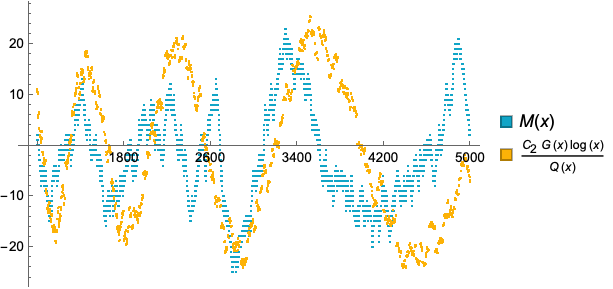
\includegraphics[width=\textwidth]{images/Figure3-CompBetweenMxAndGInvx-GInvFunctionSequenceCalculations.png}}
\captionsetup{justification=centering}
\caption{}
\end{subfigure}

\smallskip

\begin{subfigure}[t!]{0.9\textwidth}
\fbox{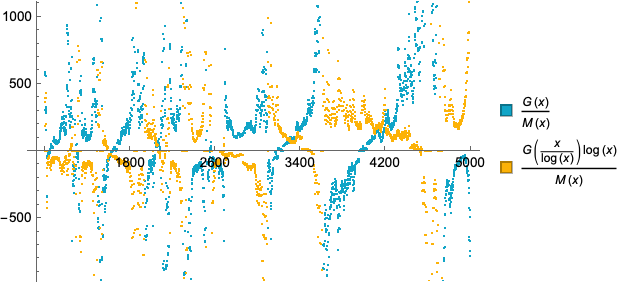
\includegraphics[width=\textwidth]{images/Figure6-RatiosOfGInvToMxAndScaledVersions-GInvFunctionSequenceCalculations.png}}
\captionsetup{justification=centering}
\caption{}
\end{subfigure}

\captionsetup{justification=centering}
\caption{} 
\label{figure_MxAndNewAuxPartialSums_Comparison_Intro_v2_v1} 

\end{figure} 

\begin{figure}[ht!]

\captionsetup{singlelinecheck=off}
\centering

\begin{subfigure}[t!]{0.9\textwidth}
\fbox{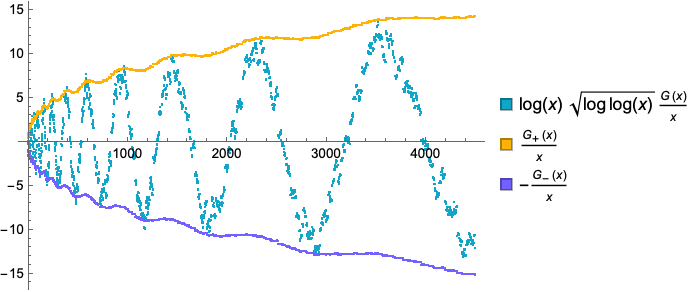
\includegraphics[width=\textwidth]{images/Figure4-ComponentsOfGInvx-GInvFunctionSequenceCalculations.png}}
\captionsetup{justification=centering}
\caption{}
\end{subfigure}

\smallskip

\begin{subfigure}[t!]{0.9\textwidth}
\fbox{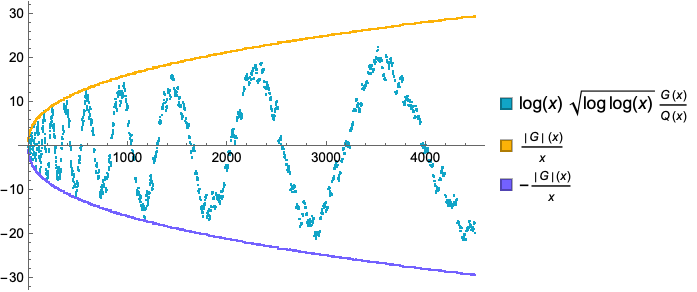
\includegraphics[width=\textwidth]{images/Figure5-ScaledGInvWithBddEnvelopes-GInvFunctionSequenceCalculations.png}}
\captionsetup{justification=centering}
\caption{}
\end{subfigure}

\captionsetup{justification=centering}
\caption{}
\label{figure_MxAndNewAuxPartialSums_Comparison_Intro_v2_v2} 

\end{figure} 

\begin{definition}
\label{def_GInvAndGInvAbs_SummFuncs_v2}
\begin{subequations}
The summatory functions of $g(n)$ and $|g(n)|$, respectively, are 
defined for all $x \geq 1$ by the partial sums 
\begin{align*}
G(x) & := \sum_{n \leq x} g(n) = \sum_{n \leq x} \lambda(n) |g(n)|, 
	\text{ and } 
	|G|(x) := \sum_{n \leq x} |g(n)|. 
\end{align*}
\end{subequations}
\end{definition}

\begin{proof}[Proof of 
              \eqref{prop_Mx_SBP_IntegralFormula_PartA} and \eqref{prop_Mx_SBP_IntegralFormula_PartB} of 
              Theorem \hlocalref{prop_Mx_SBP_IntegralFormula}] 
By applying Theorem \hlocalref{theorem_SummatoryFuncsOfDirCvls} to 
equation \eqref{eqn_AntiqueDivisorSumIdent} we have that 
\begin{align} 
\notag
M(x) & = \sum_{k=1}^{x} \left(\pi\left(\Floor{x}{k}\right)+1\right) g(k) \\ 
\notag 
     & = G(x) + \sum_{k=1}^{\frac{x}{2}} \pi\left(\Floor{x}{k}\right) g(k) \\ 
\notag 
     & = G(x) + G\left(\Floor{x}{2}\right) + 
     \sum_{k=1}^{\frac{x}{2}-1} \left( 
     \pi\left(\Floor{x}{k}\right) - \pi\left(\Floor{x}{k+1}\right) 
	\right) G(k).
\end{align} 
The upper bound on the sum is truncated to $k \in \left[1, \frac{x}{2}\right]$ in the second equation 
above because $\pi(1) = 0$. 
The third formula above follows directly by summation by parts. 
\end{proof} 
\begin{proof}[Proof of \eqref{eqn_RmkInitialConnectionOfMxToGInvx_ProvedByInversion_v1} of 
	      Theorem \hlocalref{prop_Mx_SBP_IntegralFormula}]
Lemma \hlocalref{lemma_AnExactFormulaFor_gInvByMobiusInv_v1} shows that 
\[
G(x) = \sum_{d \leq x} \lambda(d) C_{\Omega}(d) M\left(\Floor{x}{d}\right). 
\]
The identity in \eqref{eqn_AntiqueDivisorSumIdent} implies 
$$\lambda(d) C_{\Omega}(d) = (g \ast 1)(d) = (\chi_{\mathbb{P}} + \varepsilon)^{-1}(d).$$ 
We recover the stated result from the classical inversion of summatory functions in 
equation \eqref{eqn_ApostolStmt_ClassicSummatoryFuncInvThm_v1}. 
\end{proof}

\subsection{Plots and numerical experiments}

The plots shown in the figures in this section compare 
the values of $M(x)$ and $G(x)$ with scaled forms of related auxiliary partial sums: 
\begin{itemize}[noitemsep,topsep=0pt,leftmargin=0.23in]

\item In Figure \hlocalref{figure_MxAndNewAuxPartialSums_Comparison_Intro_v2_v1}, 
      we plot comparisons of $M(x)$ to scaled forms of $G(x)$ for $x \leq 5000$. The 
      absolute constant $C_2 := \zeta(2)$ and where the function 
      $Q(x) := \sum_{n \leq x} \mu^2(n)$ counts the number of squarefree integers $n \leq x$ for any 
      $x \geq 1$. In (a) the shift to the left on the $x$-axis of the former function 
      is compared and seen to be similar in shape to the magnitude of $M(x)$ on this initial subinterval. 
      It is unknown whether the similar shape and magnitude of these two functions persists for 
      much larger $x$. 
      In (b) we have observed unusual reflections and symmetry between the two ratios plotted in the 
      figure. We have numerically modified the plot values to shift the denominators of 
      $M(x)$ by one at each $x \leq 5000$ for which $M(x) = 0$. 

\item In Figure \hlocalref{figure_MxAndNewAuxPartialSums_Comparison_Intro_v2_v2}, we compare 
      envelopes on the logarithmically scaled values of $G(x) x^{-1}$ to other variants of 
      the partial sums of $g(n)$ for $x \leq 4500$. 
      In (a) we define $G(x) := G_{+}(x) - G_{-}(x)$ where the functions 
      $G_{+}(x) > 0$ and $G_{-}(x) > 0$ for all $x \geq 1$, 
      i.e., the signed component functions $G_{\pm}(x)$ 
      denote the unsigned contributions of only those summands 
      $|g(n)|$ over $n \leq x$ where $\lambda(n) = \pm 1$, respectively. 
      The summatory function $Q(x) = \frac{6x}{\pi^2}\left(1+O\left(\frac{1}{\sqrt{x}}\right)\right)$ 
      in (b) has the same definition as in 
      Figure \hlocalref{figure_MxAndNewAuxPartialSums_Comparison_Intro_v2_v1} above. 
      The second plot suggests that for large $x$ 
      \[
      |G(x)| \ll \frac{|G|(x)}{(\log x) \sqrt{\log\log x}} = 
           \frac{1}{(\log x) \sqrt{\log\log x}} \times \sum_{n \leq x} |g(n)|.
      \]

\end{itemize}

\subsection{Local cancellation in 
	    the new formulas for the Mertens function} 
\label{subSection_LocalCancellationOfGInvx} 

\begin{definition}
Let $p_n$ denote the $n^{th}$ prime for $n \geq 1$ 
\cite[\seqnum{A000040}]{OEIS}. 
The set of primorial integers is defined by  
\cite[\seqnum{A002110}]{OEIS} 
\[
\left\{n\#\right\}_{n \geq 1} = \left\{\prod_{k=1}^{n} p_k\right\}_{n \geq 1}. 
\]
\end{definition}

\begin{prop}
\label{theorem_PrimorialSeqGInvCalcs_v1} 
As $m \rightarrow \infty$, each of the following holds: 
\begin{align} 
\tag{A} 
-G((4m+1)\#) & \asymp (4m+1)!, \\ 
\tag{B} 
G\left(\frac{(4m+1)\#}{p_k}\right) & \asymp (4m)!, 
     \text{ for any } 1 \leq k \leq 4m+1. 
\end{align} 
\end{prop}
\begin{proof} 
We have by \eqref{eqn_PropB_lemma_gInv_MxExample} 
that for all squarefree integers $n \geq 1$ 
\begin{align*} 
|g(n)| & = \sum_{j=0}^{\omega(n)} \binom{\omega(n)}{j} \times j! 
     = (\omega(n))! \times \sum_{j=0}^{\omega(n)} \frac{1}{j!} \\ 
     & = (\omega(n))! \times \left(e + O\left(\frac{1}{(\omega(n)+1)!}\right)\right). 
\end{align*} 
Let $m$ be a large positive integer. 
We obtain main terms of the form 
\begin{align} 
\label{eqn_proof_tag_GinvxLocalCancellation_v1} 
\sum_{\substack{n \leq (4m+1)\# \\ \omega(n)=\Omega(n)}} \lambda(n) |g(n)| 
     & = \sum_{0 \leq k \leq 4m+1} \binom{4m+1}{k} (-1)^{k} k! 
     \left(e + O\left(\frac{1}{(k+1)!}\right)\right) \\ 
\notag 
     & = -(4m+1)! + O\left(\frac{1}{4m+1}\right). 
\end{align} 
The formula for $C_{\Omega}(n)$ stated in 
\eqref{eqn_proof_tag_hInvn_ExactNestedSumFormula_CombInterpetIdent_v3} 
then implies the result in (A). 
This happens because the contributions from the summands of the inner 
summation on the right-hand-side of 
\eqref{eqn_proof_tag_GinvxLocalCancellation_v1} 
off of the squarefree integers 
are at most a bounded multiple of $(-1)^k \times k!$ when $\Omega(n) = k$. 
We can similarly derive that for any $1 \leq k \leq 4m+1$ 
\begin{align*}
G\left(\frac{(4m+1)\#}{p_k}\right) & \asymp \sum_{0 \leq k \leq 4m} \binom{4m}{k} (-1)^{k} k! 
     \left(e + O\left(\frac{1}{(k+1)!}\right)\right) = (4m)! + O\left(\frac{1}{4m+1}\right). 
     \qedhere 
\end{align*}
\end{proof}

\begin{remark}
\label{remark_LocalCancellationWithGxAlongThePrimorialsUnderTheRH} 
The Riemann hypothesis (RH) is equivalent to showing that 
\begin{equation} 
\label{eqn_MertensMx_RHEquivProblem_Stmt_intro} 
M(x) = O\left(x^{\frac{1}{2}+\epsilon}\right), \text{ for all } 0 < \epsilon < \frac{1}{2}.
\end{equation}
We expect that there is usually (almost always) 
a large amount cancellation between the successive 
values of the summatory function in 
\eqref{eqn_RmkInitialConnectionOfMxToGInvx_ProvedByInversion_v1}. 
Proposition \hlocalref{theorem_PrimorialSeqGInvCalcs_v1} 
demonstrates the phenomenon well along the infinite 
subsequence of the primorials $\{(4m+1)\#\}_{m \geq 1}$. 
If the RH is true, the sums of the leading constants with opposing signs 
on the asymptotic bounds for the functions from the last proposition 
are necessarily required to match. 
In particular, we have that 
\cite{DUSART-1999,DUSART-2010} 
\[
n\# \sim e^{\vartheta(p_n)} \asymp n^n (\log n)^n e^{-n(1+o(1))}, 
     \text{ as } n \rightarrow \infty. 
\]
The observation on the necessary cancellation in 
\eqref{eqn_RmkInitialConnectionOfMxToGInvx_ProvedByInversion_v1}
then follows from the fact that if we obtain a contrary result  
\[
\frac{M((4m+1)\#)}{\sqrt{(4m+1)\#}} \gg \left[(4m+1)\#\right]^{\delta_0}, 
     \text{ as } m \rightarrow \infty, 
\]
for some fixed $\delta_0 > 0$. 
If the last equation were to hold, we would find a contradiction to the 
condition required by equation \eqref{eqn_MertensMx_RHEquivProblem_Stmt_intro}. 
Assuming the RH, we can state a stronger bound for the 
Mertens function along this subsequence by considering the 
error terms given in the proof of 
Proposition \hlocalref{theorem_PrimorialSeqGInvCalcs_v1}. 
\end{remark}

\section{Conclusions}

\subsection{Summary}

We have identified a sequence, 
$\{g(n)\}_{n \geq 1}$, that is the Dirichlet inverse of the 
shifted strongly additive function $\omega(n)$. 
There is a natural 
combinatorial interpretation to the repetition of distinct values 
of $|g(n)|$ in terms of the configuration of the 
exponents in the prime factorization of any $n \geq 2$. 
The sign of $g(n)$ is given by $\lambda(n)$ for all $n \geq 1$. 
This leads to a new exact relations of the 
summatory function $G(x)$ to $M(x)$ and the classical partial sums $L(x)$. 
We have formalized a new perspective from which we might express 
our intuition about features of the distribution of $G(x)$ 
via the properties of its $\lambda(n)$-sign-weighted summands.
The new results proved within this article 
are significant in providing a new window through which we can view bounding $M(x)$ 
through asymptotics of the unsigned sequences and their partial sums. 

\subsection{Discussion of the new results}

Probabilistic models of the M\"obius function lead us to consider the behavior of $M(x)$ 
as a sum of independent and identically distributed (i.i.d.) random variables. 
Suppose that $\{X_n\}_{n \geq 1}$ is a sequence of i.i.d. random variables 
such that for all $n \geq 1$ 
$$\mathbb{P}[X_n = 1] = \frac{3}{\pi^2}, \mathbb{P}[X_n = 0] = 1 - \frac{6}{\pi^2}, \text{ and }  
  \mathbb{P}[X_n = -1] = \frac{3}{\pi^2},$$ 
i.e., so that the sequence provides a randomized model of the values of $\mu(n)$ on the average. 
Under the assumption of this model, we may approximate the partial sums as 
$M(x) \cong \sum_{n \leq x} X_n$. 
This viewpoint models predictions of certain limiting asymptotic behavior of the 
Mertens function such as 
\[
\mathbb{E}\left[\sum_{1 \leq n \leq x} X_n\right] = 0, 
     \operatorname{Var}\left(\sum_{1 \leq n \leq x} X_n\right) = \frac{6x}{\pi^2}, 
     \text{ and } 
     \limsup_{x \rightarrow \infty} \frac{\left\lvert \sum\limits_{1 \leq n \leq x} X_n 
     \right\rvert}{\sqrt{x \log\log x}} = \frac{2\sqrt{3}}{\pi}
     \text{ (almost surely).} 
\]
The property of the symmetry of the distinct values of $|g(n)|$ with respect to the 
prime factorizations of $n \geq 2$ in \eqref{eqn_FactSymmPropertyOfgn_v1} 
shows that the unsigned weights on $\lambda(n)$ in 
the new formulas Theorem \hlocalref{prop_Mx_SBP_IntegralFormula} 
are comparatively easier to work with than the known 
exact expressions for $M(x)$ like equation \eqref{eqn_MxInTermsOfLx_v1}. 

Finding tight bounds on the distribution of 
$L(x)$ is a problem that is equally as difficult 
as understanding the properties of $M(x)$
along infinite subsequences (\cf \cite{MR2877066,MR3779960,TAO-LOGAVGD-CHOWLA}). 
Indeed, $\lambda(n) = \mu(n)$ for all squarefree $n \geq 1$ so that 
$\lambda(n)$ agrees with $\mu(n)$ at most large $n$ as the asymptotic density of the 
squarefree integers is positive. 
We should infer that $\lambda(n)$ must then inherit the pseudo-randomized quirks 
of $\mu(n)$ predicted by models of this function in Sarnak's conjecture. 
On the other hand, arguments for why the formulas in 
Theorem \hlocalref{prop_Mx_SBP_IntegralFormula} are more desirable to explore than 
other classical formulae for $M(x)$ have the following counter points:
\begin{itemize}[noitemsep,topsep=0pt,leftmargin=0.23in]
\item Breakthrough work in recent years due to 
	Matom\"aki, Radziwi{\l\l} and Soundararajan to 
	bound multiplicative functions 
	in short intervals has 
	proven fruitful when applied to $\lambda(n)$ 
	\cite{SOUND-LLAMBDA-SHORT-INTS,MATRADZE-MULTFUNCS-SHORT-INTS}. 
	The analogs of results of this type corresponding 
	to the M\"obius function are not clearly attained; 
\item The squarefree $n \geq 1$ on which $\lambda(n)$ and $\mu(n)$ must identically agree 
	are in some senses easier integer cases to handle 
	insomuch as we can prove very regular properties 
	that govern the distributions of the distinct values of 
	$\omega(n)$, $\Omega(n)$ and their difference over $n \leq x$ as $x \rightarrow \infty$ 
	\citep[\cf \S 2.4; \S 7.4]{MV}; 
\item The function $\lambda(n)$ is completely 
	multiplicative. Hence, sign weighting by the function $\lambda(n)$ may eventually reflect 
	a nicer cousin to the multiplicative $\mu(n)$ along the 
	integers $n \geq 4$ for which $\mu(n) = 0$. 
	This idea, and applications to bounding $M(x)$ via $G(x)$ in 
	equation \eqref{eqn_RmkInitialConnectionOfMxToGInvx_ProvedByInversion_v1}, 
	are stated imprecisely for now.
\end{itemize}

\renewcommand{\refname}{References} 
\addcontentsline{toc}{section}{References}
%\bibliography{glossaries-bibtex/thesis-references}{}
\bibliographystyle{plain}

\begin{thebibliography}{10}

\bibitem{APOSTOLANUMT}
T.~M. Apostol.
\newblock {\em Introduction to Analytic Number Theory}.
\newblock Springer--Verlag, 1976.

\bibitem{ANT-BATEMAN-DIAMOND}
P.~T. Bateman and H.~G. Diamond.
\newblock {\em Analytic Number Theory}.
\newblock World Scientific Publishing, 2004.

\bibitem{BILLINGSLY-CLT-PRIMEDIVFUNC}
P.~Billingsley.
\newblock On the central limit theorem for the prime divisor function.
\newblock {\em Amer. Math. Monthly}, 76(2):132--139, 1969.

\bibitem{BILLINGSLY-PROB-AND-MEASURE-BOOK}
P.~Billingsley.
\newblock {\em Probability and measure}.
\newblock Wiley, third edition, 1994.

\bibitem{DUSART-1999}
P.~Dusart.
\newblock The $k^{th}$ prime is greater than $k(\log k +\log\log k-1)$ for $k
  \geq 2$.
\newblock {\em Math. Comp.}, 68(225):411--415, 1999.

\bibitem{DUSART-2010}
P.~Dusart.
\newblock Estimates of some functions over primes without {R}.{H}., 2010.

\bibitem{ERDOS-KAC-REF}
P.~Erd{\H{o}}s and M.~Kac.
\newblock The {G}aussian errors in the theory of additive arithmetic functions.
\newblock {\em American Journal of Mathematics}, 62(1):738--742, 1940.

\bibitem{MR3779960}
N.~Frantzikinakis and B.~Host.
\newblock The logarithmic {S}arnak conjecture for ergodic weights.
\newblock {\em Ann. of Math. (2)}, 187(3):869--931, 2018.

\bibitem{FROBERG-1968}
C.~E. Fr{\"{o}}berg.
\newblock On the prime zeta function.
\newblock {\em BIT Numerical Mathematics}, 8:87--202, 1968.

\bibitem{MR2877066}
B.~Green and T.~Tao.
\newblock The {M}\"{o}bius function is strongly orthogonal to nilsequences.
\newblock {\em Ann. of Math. (2)}, 175(2):541--566, 2012.

\bibitem{HARDYWRIGHT}
G.~H. Hardy and E.~M. Wright, editors.
\newblock {\em An Introduction to the Theory of Numbers}.
\newblock Oxford University Press, 2008 (Sixth Edition).

\bibitem{HUMPHRIES-JNT-2013}
P.~Humphries.
\newblock The distribution of weighted sums of the {L}iouville function and
  {P}\'{o}lya's conjecture.
\newblock {\em J. Number Theory}, 133:545--582, 2013.

\bibitem{LEHMAN-1960}
R.~S. Lehman.
\newblock On {L}iouville's function.
\newblock {\em Math. Comput.}, 14:311--320, 1960.

\bibitem{MATRADZE-MULTFUNCS-SHORT-INTS}
K.~Matom{\"{a}}ki and M.~Radziwi{\l\l}.
\newblock Multiplicative functions in short intervals.
\newblock {\em Ann. of Math.}, 183:1015--1056, 2016.

\bibitem{MV}
H.~L. Montgomery and R.~C. Vaughan.
\newblock {\em Multiplicative Number Theory: I. Classical Theory}.
\newblock Cambridge, 2006.

\bibitem{NEMES2015C}
G.~Nemes.
\newblock The resurgence properties of the incomplete gamma function {II}.
\newblock {\em Stud. Appl. Math.}, 135(1):86--116, 2015.

\bibitem{NEMES2016}
G.~Nemes.
\newblock The resurgence properties of the incomplete gamma function {I}.
\newblock {\em Anal. Appl. (Singap.)}, 14(5):631--677, 2016.

\bibitem{NEMES2019}
G.~Nemes and A.~B.~Olde Daalhuis.
\newblock Asymptotic expansions for the incomplete gamma function in the
  transition regions.
\newblock {\em Math. Comp.}, 88(318):1805--1827, 2019.

\bibitem{NISTHB}
F.~W.~J. Olver, D.~W. Lozier, R.~F. Boisvert, and C.~W. Clark, editors.
\newblock {\em {NIST} Handbook of Mathematical Functions}.
\newblock Cambridge University Press, 2010.

\bibitem{LOG-COMB-STRUCTS-BOOK}
A.~D.~Barbour R.~Arratia and Simon Tavar{\'{e}}.
\newblock {\em Logarithmic Combinatorial Structures: A Probabilistic Approach}.
\newblock Preprint draft, 2002.

\bibitem{OEIS}
N.~J.~A. Sloane.
\newblock The {O}nline {E}ncyclopedia of {I}nteger {S}equences, 2021.
\newblock \url{http://oeis.org}.

\bibitem{SOUND-LLAMBDA-SHORT-INTS}
K.~Soundararajan.
\newblock The {L}iouville function in short intervals (after {M}atomaki and
  {R}adziwi{\l}{\l}).
\newblock {\em arXiv:1606.08021}, 2016.

\bibitem{TAO-LOGAVGD-CHOWLA}
T.~Tao.
\newblock The logarithmically averaged {C}howla and {E}lliott conjectures for
  two-point correlations.
\newblock {\em Forum of Mathematics}, 4:e8, 2016.

\end{thebibliography}

\newpage
\appendix
\cftaddtitleline{toc}{section}{Appendices on supplementary material}{}
\setcounter{section}{0} 
\renewcommand{\thesection}{\Alph{section}} 

\section{Glossary of notation and conventions}
\label{Section_NotationAndConventions}

\renewcommand*{\glsclearpage}{}
\renewcommand{\glossarysection}[2][]{}
\printglossary[type={symbols},
               style={glossstyleSymbol},
               nogroupskip=true]

\section{The distributions of $\omega(n)$ and $\Omega(n)$} 
\label{subSection_TheKnownDistsOfThePrimeOmegaFunctions_IntroResults_v1} 

As $n \rightarrow \infty$, we have that 
$$\frac{1}{n} \times \sum_{k \leq n} \omega(k) = \log\log n + B_1 + o(1),$$ 
and 
$$\frac{1}{n} \times \sum_{k \leq n} \Omega(k) = \log\log n + B_2 + o(1),$$ for 
$B_1 \approx 0.261497$ and $B_2 \approx 1.03465$ 
absolute constants \cite[\S 22.10]{HARDYWRIGHT}. 
The next theorems reproduced from \cite[\S 7.4]{MV} bound the frequency of the 
number of $\omega(n)$ and $\Omega(n)$ over $n \leq x$ such that 
these functions diverge substantially from their average order 
(\cf \cite{ERDOS-KAC-REF,BILLINGSLY-CLT-PRIMEDIVFUNC} \cite[\S 7.4]{MV}). 

\begin{theorem} 
\label{theorem_MV_Thm7.20-init_stmt} 
For $x \geq 2$ and $r > 0$, let 
\begin{align*} 
A(x, r) & := \#\left\{n \leq x: \Omega(n) \leq r \log\log x\right\}, \\ 
B(x, r) & := \#\left\{n \leq x: \Omega(n) \geq r \log\log x\right\}. 
\end{align*} 
If $0 < r \leq 1$, then 
\[
A(x, r) \ll\phantom{_R} x (\log x)^{r-1 - r\log r}, \text{ as } x \rightarrow \infty. 
\]
If $1 \leq r \leq R < 2$, then 
\[
B(x, r) \ll_R x (\log x)^{r-1-r \log r}, \text{ as } x \rightarrow \infty. 
\]
\end{theorem} 

\begin{theorem}
\label{theorem_HatPi_ExtInTermsOfGz} 
For integers $k \geq 1$ and $x \geq 2$ 
$$\widehat{\pi}_k(x) := \#\{2 \leq n \leq x: \Omega(n)=k\}.$$ 
For $0 < R < 2$, uniformly for $1 \leq k \leq R \log\log x$ 
\[
\widehat{\pi}_k(x) = \frac{x}{\log x} \times \mathcal{G}\left(\frac{k-1}{\log\log x}\right) 
     \frac{(\log\log x)^{k-1}}{(k-1)!} \left(1 + O_R\left(\frac{k}{(\log\log x)^2}\right)\right), 
     \text{ as } x \rightarrow \infty, 
\]
where 
\[
\mathcal{G}(z) := \frac{1}{\Gamma(1+z)} \times 
	\prod_p \left(1-\frac{z}{p}\right)^{-1} \left(1-\frac{1}{p}\right)^z, 
	\text{ for } 0 \leq |z| < R. 
\]
\end{theorem} 

We can extend the work in \cite{MV} on the distribution of $\Omega(n)$ to obtain 
corresponding analogous results for the distribution of $\omega(n)$. 

\begin{remark} 
\label{remark_MV_Pikx_FuncResultsAnnotated_v1} 
For integers $k  \geq 1$ and $x \geq 2$, we define 
\[
\pi_k(x) := \#\{2 \leq n \leq x: \omega(n)=k\}.
\]
For $0 < R < 2$ and as $x \rightarrow \infty$ 
\begin{equation}
\label{eqn_Pikx_UniformAsymptoticsStmt_from_MV_v2} 
\pi_k(x) = \frac{x}{\log x} \times 
     \widetilde{\mathcal{G}}\left(\frac{k-1}{\log\log x}\right) 
     \frac{(\log\log x)^{k-1}}{(k-1)!} \left( 
     1 + O_R\left(\frac{k}{(\log\log x)^2}\right) 
     \right), 
\end{equation}
uniformly for $1 \leq k \leq R\log\log x$. 
The factor involving the function $\widetilde{\mathcal{G}}(z)$ is 
defined by $\widetilde{\mathcal{G}}(z) := \widetilde{F}(1, z) \times \Gamma(1+z)^{-1}$ where 
\[
\widetilde{F}(s, z) := \prod_p \left(1 + \frac{z}{p^s-1}\right) \left(1 - \frac{1}{p^s}\right)^{z}, 
	\text{ for } \Re(s) > \frac{1}{2} \text{ and } |z| \leq R < 2. 
\]
Let the functions 
\begin{align*} 
C(x, r) & := \#\{n \leq x: \omega(n) \leq r \log\log x\}, \\ 
D(x, r) & := \#\{n \leq x: \omega(n) \geq r \log\log x\}. 
\end{align*} 
The following upper bounds hold as $x \rightarrow \infty$: 
\begin{align*} 
C(x, r) & \ll\phantom{_R} x (\log x)^{r - 1 - r \log r}, \text{ uniformly for } 0 < r \leq 1, \\ 
D(x, r) & \ll_R x (\log x)^{r - 1 - r \log r}, \text{ uniformly for } 1 \leq r \leq R < 2.
\end{align*} 
\end{remark} 

\section{Asymptotics of the incomplete gamma function} 
\label{subSection_OtherFactsAndResults} 

We cite the correspondence with Gerg\H{o} Nemes 
from the Alfr\'{e}d R\'{e}nyi Institute of Mathematics and his 
careful notes on the limiting asymptotics for the sums identified in this section. 
The communication of his proofs are adapted to establish the next lemmas based on 
\cite{NEMES2015C,NEMES2016,NEMES2019}. 

\begin{definition}
The (upper) incomplete gamma function is defined by \cite[\S 8.4]{NISTHB} 
\[
\Gamma(a, z) = \int_{z}^{\infty} t^{a-1} e^{-t} dt, \text{ for } 
	a \in \mathbb{R} \text{ and } |\arg z| < \pi.  
\]
\end{definition}

The function $\Gamma(a, z)$ can be continued to an analytic function of $z$ on the 
universal covering of $\mathbb{C} \mathbin{\backslash} \{0\}$. 
For $a \in \mathbb{Z}^{+}$, the function $\Gamma(a, z)$ is an entire function of $z$. 

\begin{facts} 
\label{facts_ExpIntIncGammaFuncs} 
\begin{subequations}
The following properties hold \cite[\S 8.4; \S 8.11(i)]{NISTHB}: 
\begin{align} 
\label{eqn_IncompleteGamma_PropA} 
     \Gamma(a, z) & = (a-1)! e^{-z} \times \sum_{k=0}^{a-1} \frac{z^k}{k!}, \text{ for } 
     a \in \mathbb{Z}^{+} \text{ and } z \in \mathbb{C}, \\ 
\label{eqn_IncompleteGamma_PropB} 
\Gamma(a, z) & \sim z^{a-1} e^{-z}, \text{ for fixed } a \in \mathbb{R} 
     \text{ and } z > 0 \text{ as } z \rightarrow \infty. 
\end{align}
For $z > 0$, as $z \rightarrow \infty$ we have that \cite{NEMES2015C} 
\begin{equation} 
\label{eqn_IncompleteGamma_PropC}
\Gamma(z, z) = \sqrt{\frac{\pi}{2}} z^{z-\frac{1}{2}} e^{-z} + 
     O\left(z^{z-1} e^{-z}\right), 
\end{equation} 
For fixed, finite real $|\rho| > 0$, we define the sequence 
$\{b_n(\rho)\}_{n \geq 0}$ by 
the following recurrence relation for $n \geq 0$: 
\[
b_n(\rho) = \rho(1-\rho) b_{n-1}^{\prime}(\rho) + \rho(2n-1) b_{n-1}(\rho) + \delta_{n,0}. 
\]
If $z,a \rightarrow \infty$ with $z = \rho a$ for some $\rho > 1$ such that 
$(\rho - 1)^{-1} = o\left(\sqrt{|a|}\right)$, then \cite{NEMES2015C}
\begin{equation}
\label{eqn_IncompleteGamma_PropD}
\Gamma(a, z) \sim z^a e^{-z} \times \sum_{n \geq 0} \frac{(-a)^n b_n(\rho)}{(z-a)^{2n+1}}. 
\end{equation} 
\end{subequations}
\end{facts} 

\begin{prop}
\label{prop_IncGammaLambdaTypeBounds_v1}
\begin{subequations}
Let $a,z,\rho$ be positive real parameters such that $z=\rho a$. 
If $\rho \in (0, 1)$, then as $z \rightarrow \infty$ 
\begin{equation}
\Gamma(a, z) = \Gamma(a) + O_{\rho}\left(z^{a-1} e^{-z}\right). 
\end{equation}
If $\rho > 1$, then as 
$z \rightarrow \infty$ 
\begin{equation}
\Gamma(a, z) = \frac{z^{a-1} e^{-z}}{1-\rho^{-1}} + O_{\rho}\left(z^{a-2} e^{-z}\right). 
\end{equation}
If $\rho > W(1)$, then as $z \rightarrow \infty$ 
\begin{equation}
\Gamma(a, z e^{\pm\pi\imath}) = -e^{\pm \pi\imath a} \frac{z^{a-1} e^{z}}{1 + \rho^{-1}} + 
     O_{\rho}\left(z^{a-2} e^{z}\right). 
\end{equation}
\end{subequations}
\end{prop}

\begin{remark}
The first two estimates in the proposition 
are only useful when $\rho$ is bounded away from the transition point at one. 
We cannot write the last expansion above 
as $\Gamma(a, -z)$ directly unless $a \in \mathbb{Z}^{+}$ 
as the incomplete gamma function 
has a branch point at the origin with respect to its second variable. 
This function becomes a single-valued 
analytic function of its second input by continuation 
on the universal covering of $\mathbb{C} \mathbin{\backslash} \{0\}$. 
\end{remark}

\begin{proof}[Proof of Proposition \hlocalref{prop_IncGammaLambdaTypeBounds_v1}] 
The first asymptotic estimate follows directly from the following 
asymptotic series expansion that holds as $z \rightarrow \infty$ 
\cite[Eq.\ (2.1)]{NEMES2019}: 
\[
\Gamma(a, z) \sim \Gamma(a) + z^a e^{-z} \times \sum_{k \geq 0} 
     \frac{(-a)^k b_k(\rho)}{(z-a)^{2k+1}}. 
\]
Using the notation from \eqref{eqn_IncompleteGamma_PropD} and \cite{NEMES2016} 
\[
\Gamma(a, z) = \frac{z^{a-1} e^{-z}}{1-\rho^{-1}} + z^{a} e^{-z} R_1(a, \rho). 
\]
From the bounds in \cite[\S 3.1]{NEMES2016}, we have 
\[
\left\lvert z^{a} e^{-z} R_1(a, \rho) \right\rvert \leq 
     z^a e^{-z} \times \frac{a \cdot b_1(\rho)}{(z-a)^{3}} = 
     \frac{z^{a-2} e^{-z}}{(1-\rho^{-1})^{3}}
\]
The main and error terms in the previous equation can also be 
seen by applying the asymptotic series in 
\eqref{eqn_IncompleteGamma_PropD} directly. 

The proof of the third equation above follows from the asymptotics 
\cite[Eq.\ (1.1)]{NEMES2015C}
\[
\Gamma(-a, z) \sim z^{-a} e^{-z} \times \sum_{n \geq 0} \frac{a^n b_n(-\rho)}{(z+a)^{2n+1}}, 
\]
by setting $(a, z) \mapsto \left(a e^{\pm \pi\imath}, z e^{\pm \pi\imath}\right)$ so that 
$\rho = \frac{z}{a} > W(1) \approx 0.56714$. 
The restriction on the range of $\rho$ over which the third formula holds is made to ensure that 
the formula from the reference is valid at negative real $a$. 
\end{proof}

\section{Inversion theorems for partial sums of Dirichlet convolutions}
\label{Section_PrelimProofs_Config} 
\label{subSection_PrelimProofs_Config_InversionTheorem}

\begin{proof}[Proof of Theorem \hlocalref{theorem_SummatoryFuncsOfDirCvls}] 
\label{proofOf_theorem_SummatoryFuncsOfDirCvls} 
Suppose that $h,r$ are arithmetic functions such that $r(1) \neq 0$. 
The following formulas hold for all $x \geq 1$: 
\begin{align} 
\notag 
S_{r \ast h}(x) & := \sum_{n=1}^{x} \sum_{d|n} r(n) h\left(\frac{n}{d}\right) = 
     \sum_{d=1}^x r(d) H\left(\floor{\frac{x}{d}}\right) \\ 
\label{eqn_proof_tag_PigAsthx_ExactSummationFormula_exp_v2} 
     & \phantom{:} = 
     \sum_{i=1}^x \left(R\left(\floor{\frac{x}{i}}\right) - R\left(\floor{\frac{x}{i+1}}\right)\right) H(i). 
\end{align} 
The first formula on the right-hand-side above is well known from the references. 
The second formula is justified directly using 
summation by parts as \cite[\S 2.10(ii)]{NISTHB} 
\begin{align*} 
S_{r \ast h}(x) & = \sum_{d=1}^x h(d) R\left(\floor{\frac{x}{d}}\right) \\ 
     & = \sum_{i \leq x} \left(\sum_{j \leq i} h(j)\right) \times 
     \left(R\left(\floor{\frac{x}{i}}\right) - 
     R\left(\floor{\frac{x}{i+1}}\right)\right). 
\end{align*} 
We form the invertible matrix of coefficients, denoted by $\hat{R}$ below, 
associated with the linear system defining $H(j)$ for 
$1 \leq j \leq x$ in \eqref{eqn_proof_tag_PigAsthx_ExactSummationFormula_exp_v2} by defining
\[
R_{x,j} := R\left(\Floor{x}{j}\right) \Iverson{j \leq x}, 
\]
and 
\[
r_{x,j} := R_{x,j} - R_{x,j+1}, \text{ for } j \geq 1. 
\] 
Since $r_{x,x} = R(1) = r(1) \neq 0$ for all $x \geq 1$ and $r_{x,j} = 0$ for all $j > x$, 
the matrix we have defined in this problem is lower triangular with a non-zero 
constant on its diagonals, and so is invertible. 
If we let $\hat{R} := (R_{x,j})$, then the next matrix is 
expressed by applying an invertible shift operation as 
\[
(r_{x,j}) = \hat{R} \left(I - U^{T}\right). 
\]
The $N \times N$ square matrix $U$ 
has $(i,j)^{th}$ entries for all $1 \leq i,j \leq N$ when $N \geq x$ that are defined by 
$(U)_{i,j} = \delta_{i+1,j}$ so that 
\[
\left[\left(I - U^T\right)^{-1}\right]_{i,j} = \Iverson{j \leq i}. 
\]
We observe the identity 
\[
\Floor{x}{j} - \Floor{x-1}{j} = \begin{cases} 
     1, & \text{ if $j|x$; } \\ 
     0, & \text{ otherwise. } 
     \end{cases} 
\] 
The previous equation implies that 
\begin{equation} 
\label{eqn_proof_tag_FloorFuncDiffsOfSummatoryFuncs_v2} 
R\left(\floor{\frac{x}{j}}\right) - R\left(\floor{\frac{x-1}{j}}\right) = 
     \begin{cases} 
     r\left(\frac{x}{j}\right), & \text{ if $j | x$; } \\ 
     0, & \text{ otherwise. } 
     \end{cases}
\end{equation} 
We use the property in \eqref{eqn_proof_tag_FloorFuncDiffsOfSummatoryFuncs_v2} 
to shift the matrix $\hat{R}$, and then invert the result to obtain a matrix involving the 
Dirichlet inverse of $r$ as 
\begin{align*} 
\left(\left(I-U^{T}\right) \hat{R}\right)^{-1} & = 
     \left(r\left(\frac{x}{j}\right) \Iverson{j|x}\right)^{-1} = 
     \left(r^{-1}\left(\frac{x}{j}\right) \Iverson{j|x}\right). 
\end{align*} 
Our target matrix in the inversion problem is 
$$(r_{x,j}) = \left(I-U^{T}\right) \left(r\left(\frac{x}{j}\right) \Iverson{j|x}\right) \left(I-U^{T}\right)^{-1}.$$
We can express its inverse by a similarity transformation conjugated by shift operators by expanding 
\begin{align*} 
(r_{x,j})^{-1} & = \left(I-U^{T}\right)^{-1} \left(r^{-1}\left(\frac{x}{j}\right) 
     \Iverson{j|x}\right) \left(I-U^{T}\right) \\ 
     & = \left(\sum_{k=1}^{\floor{\frac{x}{j}}} r^{-1}(k)\right) \left(I-U^{T}\right) \\ 
     & = \left(\sum_{k=1}^{\floor{\frac{x}{j}}} r^{-1}(k) - \sum_{k=1}^{\floor{\frac{x}{j+1}}} r^{-1}(k)\right). 
\end{align*} 
The summatory function $H(x)$ is given exactly for any integers $x \geq 1$ 
by a vector product with the inverse matrix from the previous equation as 
\begin{align*} 
H(x) & = \sum_{k=1}^x \left(\sum_{j=\floor{\frac{x}{k+1}}+1}^{\floor{\frac{x}{k}}} r^{-1}(j)\right) 
     \times S_{r \ast h}(k). 
\end{align*} 
We can prove a second inversion formula providing the coefficients of the summatory function 
$R^{-1}(j)$ for $1 \leq j \leq x$ from the last equation by adapting our argument to prove 
\eqref{eqn_proof_tag_PigAsthx_ExactSummationFormula_exp_v2} above. 
This leads to the following alternate identity expressing $H(x)$: 
\[
H(x) = \sum_{k=1}^{x} r^{-1}(k) \times S_{r \ast h}\left(\Floor{x}{k}\right). 
     \qedhere 
\]
\end{proof} 

\end{document}
